\documentclass[11pt,a4paper]{article}
\usepackage[margin=2.4cm,headheight=14pt]{geometry}
\usepackage{amsmath}
\usepackage{fontspec}
\usepackage{unicode-math}
\setmainfont{texgyrepagella}[Extension=.otf,UprightFont=*-regular,BoldFont=*-bold,ItalicFont=*-italic,BoldItalicFont=*-bolditalic]
\setsansfont{texgyreheros}[Extension=.otf,UprightFont=*-regular,BoldFont=*-bold]
\setmonofont{DejaVuSansMono.ttf}[Scale=0.82]
\setmathfont{texgyrepagella-math.otf}
\usepackage{xeCJK}
\setCJKmainfont{FandolSong-Regular.otf}[BoldFont=FandolHei-Bold.otf,ItalicFont=FandolKai-Regular.otf]
\setCJKsansfont{FandolHei-Regular.otf}[BoldFont=FandolHei-Bold.otf]
\setCJKmonofont{FandolFang-Regular.otf}
\xeCJKsetup{PunctStyle=quanjiao,CJKecglue={\hskip 0.15em plus 0.05em}}
\usepackage{booktabs,longtable,array,tabularx,multirow}
\usepackage{graphicx,float}
\usepackage[section]{placeins}
\usepackage{flafter}
\usepackage[font=small,labelfont=bf,labelsep=quad]{caption}
\usepackage{xcolor}
\usepackage{enumitem}
\setlist{nosep,leftmargin=1.6em}
\usepackage{fancyhdr}
\usepackage[round,authoryear]{natbib}
\usepackage[colorlinks,linkcolor={blue!50!black},citecolor={green!40!black},urlcolor={blue!60!black}]{hyperref}
\renewcommand{\abstractname}{摘\quad 要}
\renewcommand{\figurename}{图}
\renewcommand{\tablename}{表}
\renewcommand{\refname}{参考文献}
\renewcommand{\contentsname}{目\quad 录}
\renewcommand{\appendixname}{附录}
\linespread{1.18}
\setlength{\parskip}{0.35em}
\newcolumntype{Y}{>{\raggedright\arraybackslash}X}
\newcommand{\RAM}{\mathrm{RAM}}
\newcommand{\FMC}{\mathrm{FMC}}
\pagestyle{fancy}
\fancyhf{}
\fancyhead[L]{\small 沪深300 S\&P Financial Viability + SPMO 动量指数}
\fancyhead[R]{\small \thepage}
\renewcommand{\headrulewidth}{0.3pt}
\begin{document}

\title{\LARGE\bfseries 沪深300 S\&P Financial Viability + SPMO 动量指数：\\[4pt]\Large 方法、数据与 2005--2026 年历史回测}
\author{csi300-spmo-index 项目\thanks{代码、数据处理流程与全部输出见 \url{https://github.com/dongzhaohe321418-lab/csi300-spmo-index}。本文全部数字由 \texttt{python scripts/generate\_research\_report.py --latex} 自动从回测输出生成；本文仅为历史回测研究，不构成投资建议。}}
\date{2026 年 9 月 10 日}
\maketitle
\thispagestyle{empty}
\begin{abstract}
本文把 S\&P 500 Momentum Index（SPMO）的编制规则平移到 A 股大盘股，构建并回测了\textbf{沪深300 S\&P Financial Viability + SPMO 动量指数}。指数以逐日点位（point-in-time）的历史沪深300成分股为母池，按 S\&P U.S. Indices 的 Financial Viability 标准（最近一季及最近四季持续经营净利润为正）剔除亏损公司，依 S\&P Momentum 方法计算 12--1 月风险调整动量并转换为 Momentum Score，选取前 20\%（约 51 只）以自由流通市值乘以 Momentum Score 加权并施加公司权重上限，每年 3 月和 9 月调仓。规则完全固定，不做参数优化。母池由中证指数公司 67 份调样公告逐笔回推重建，财务与价格数据均只使用参考日之前已公开的信息，并由程序逐期审计。2005-09-16 至 2026-09-09，指数（价格口径）年化收益 9.83\%，沪深300为 7.68\%，年化超额 2.15\%（费后 1.65\%），Sharpe 由 0.43 升至 0.49，但年化波动（26.71\%）与最大回撤（$-$77.16\%）均高于母指数，月度超额收益的 $t$ 统计量仅 0.97。超额收益高度集中于 2017--2020 年，2007--2016 年相对强度回撤 $-$33.2\%；最大的动量崩塌发生在 2024 年 9--12 月的政策驱动急涨中。归因显示超额几乎全部来自选股（+3.1 个百分点/年），Momentum Score 加权倾斜贡献有限；本文使用的自由流通市值代理相对官方指数每年拖累约 1.1 个百分点，因此报告的策略业绩偏保守。最后，本文在相同数据上复现了 GitHub 项目 HSI300-Momentum-Strategy 的 Top-20 等权季度动量规则：其公布的 2019--2025 年年化 22.2\% 在本文数据上复现为 19.8\%；在 2005--2026 年全样本上该规则年化 13.1\%，高于本指数（全收益费后 11.8\%），但换手约为两倍，且其基于当前行业分类的行业上限在历史上是伪影。
\end{abstract}
\begin{center}\begin{minipage}{0.86\textwidth}\small\noindent\textbf{关键词：}动量因子；风险调整动量；沪深300；S\&P 500 Momentum；Financial Viability；点位数据；指数编制；动量崩塌\end{minipage}\end{center}
\newpage\tableofcontents\vspace{1em}
\section{引言}
价格动量——过去 6 至 12 个月表现较好的股票在随后数月继续领先——是被记录最多的股票横截面异象之一 \cite{jegadeesh1993,asness2013,carhart1997}。其代价同样有充分记录：动量组合的收益分布呈显著负偏，在高波动的熊市底部反弹中会出现\emph{动量崩塌} \cite{daniel2016,barroso2015}。S\&P Dow Jones Indices 的 S\&P 500 Momentum Index 是这一因子的指数化实现 \cite{spdji_momentum}：在 S\&P 500 内按 12--1 月风险调整动量打分，选取分数最高的约 20\% 股票，以市值乘以动量分数加权，每年 3 月与 9 月调仓；Invesco S\&P 500 Momentum ETF（代码 SPMO）跟踪该指数。
本文回答一个具体问题：\textbf{把这套规则原样平移到沪深300，并叠加 S\&P U.S. Indices 用于新纳入公司的 Financial Viability 盈利资格 \cite{spdji_us}，在 2005--2026 年的 A 股历史上会得到什么？}研究目的不是寻找最优参数，而是在无前视、无幸存者偏差的数据上检验一条\emph{固定}规则的长期表现、风险特征、收益来源与失效场景。为此，本文遵循四条原则：
\begin{enumerate}
\item \textbf{规则固定。}不调参、不优化前 20\% 的比例、不加入 ROE、ROIC、PE、PB、成长、杠杆、质量等任何其他因子。
\item \textbf{点位数据。}每个参考日只使用当日已存在的信息：当日有效的沪深300成分、当日之前已公告的财务报表、当日之前的价格。
\item \textbf{自动审计。}每期成分股必须在参考日与实施日确属沪深300、满足财务资格、所用财报已公告、动量窗口有足够交易日；任一违反即报错终止。
\item \textbf{可复现。}\texttt{python main.py} 一条命令完成数据获取、股票池重建、评分、选样、加权、指数计算、回测、图表与报告。
\end{enumerate}
与既有的 A 股动量研究相比，本文的贡献主要在数据工程与工程化验证：(i) 用中证指数公司 2005 年以来的全部沪深300调样公告逐日重建点位成分股，并以\emph{每一步恰好 300 只}和\emph{回推名单与官方 2005 年全名单完全一致}作为硬性校验；(ii) 用交易所除权除息参考价自建复权序列并逐事件校验；(iii) 识别并修正免费财务数据源中 2010 年以前公告日期系统性滞后的问题；(iv) 用同一指数引擎做\emph{选股 vs 加权}的归因，并用权重代理复制母指数来量化代理误差；(v) 在完全相同的数据上复现另一公开动量策略的规则，使两种设计取向的比较不受数据差异干扰。
下文结构：第 \ref{sec:method} 节给出指数编制方法与同 S\&P 官方方法的差异；第 \ref{sec:data} 节说明数据来源、点位重建与数据质量检验；第 \ref{sec:results} 节报告回测结果；第 \ref{sec:portfolio} 节分析组合特征；第 \ref{sec:attribution} 节做收益来源分解；第 \ref{sec:cost} 节讨论交易成本；第 \ref{sec:hsmo} 节与 HSI300-Momentum-Strategy 比较；第 \ref{sec:conclusion} 节总结并逐条回答研究任务书中的 17 个问题。
\section{指数构建方法}\label{sec:method}
\FloatBarrier
\subsection{母股票池：点位沪深300}
记 $U(t)$ 为交易日 $t$ 有效的沪深300成分股集合。$U(t)$ 由中证指数公司 67 份沪深300样本调整公告（41 次定期调整、26 次临时调整，生效日 2005-07-01 至 2026-06-15）自当前官方名单逐笔向后回推得到：每撤销一次调整，名单必须恰好回到 300 只；回推至 2005-07-01 的名单必须与中证公布的全名单逐只一致，否则程序报错终止。共 949 只证券在 1225 个成员区间内曾属于沪深300。参考日 $R$ 不属于 $U(R)$ 的股票资格、入选标志和权重一律置零；调仓期间被剔除出沪深300的持仓在生效日按前收盘价剔除，权重按比例分配给其余成分。
\FloatBarrier
\subsection{S\&P Financial Viability}
S\&P U.S. Indices Methodology 要求新纳入公司满足：最近一个已公布季度的 GAAP 持续经营净利润为正，且最近四个季度合计为正 \cite{spdji_us}。本文对每个参考日的全部成分股施加该条件：\begin{equation}\mathrm{NI}^{q}_{i,\,\mathrm{latest}} > 0 \quad\text{且}\quad \sum_{k=0}^{3}\mathrm{NI}^{q}_{i,\,\mathrm{latest}-k} > 0 ,\end{equation}其中 $\mathrm{NI}^{q}$ 为单季持续经营净利润。A 股映射：以利润表\emph{持续经营净利润}（\texttt{CONTINUED\_NETPROFIT}，2018 年准则格式起披露）为主，早期回退到\emph{净利润}（\texttt{NETPROFIT}）；中国季报为年初累计数，单季值取相邻累计数之差（一季度即累计数）。只有首次公告日 $\leq R$ 的报表可用，四个连续已公布季度不足者不合格。公告日期的处理见第 \ref{sec:fin} 节。
\FloatBarrier
\subsection{SPMO 风险调整动量、$Z$ 分数与 Momentum Score}
按 S\&P Momentum Indices Methodology \cite{spdji_momentum}，对参考日 $R$、股票 $i$：\begin{align}\mathrm{Mom}_i &= \frac{P_i(R - 1\mathrm{M})}{P_i(R - 13\mathrm{M})} - 1, &\sigma_i &= \operatorname{StdDev}\bigl\{r_{i,d}: d \in (R-13\mathrm{M},\, R-1\mathrm{M}]\bigr\}, \\\RAM_i &= \mathrm{Mom}_i / \sigma_i, &Z_i &= \operatorname{clip}\!\left(\frac{\RAM_i - \overline{\RAM}}{s_{\RAM}},\, -3,\, 3\right), \\S_i &= \begin{cases} 1 + Z_i, & Z_i > 0 \\ 1/(1 - Z_i), & Z_i \leq 0 \end{cases}\end{align}其中 $P$ 为除权除息复权后的价格收益序列，日期按 A 股交易日历对齐，$r_{i,d}$ 为窗口内日收益率；窗口内交易日不足 150 天的股票不参与。均值与标准差在\emph{沪深300成分且财务合格}的股票间横截面计算。
\FloatBarrier
\subsection{选样与缓冲}
目标数量 $N^\ast = \operatorname{round}(0.2\times$ 合格且动量可计算的成分股数$)$，历史上为 45--55 只而非固定 60 只。按 S\&P 缓冲规则：$S_i$ 排名前 $0.8N^\ast$ 的股票自动入选，现有成分股排名在 $1.2N^\ast$ 以内的保留，其余按排名补足。母指数成员资格优先——被沪深300剔除的股票不能靠缓冲留任。历史上平均每期 5.9 只靠缓冲留任。
\FloatBarrier
\subsection{权重}
原始权重 $\tilde w_i = \FMC_i S_i / \sum_j \FMC_j S_j$，其中 $\FMC$ 为自由流通市值。随后施加公司权重上限\begin{equation} c_i = \min\bigl(9\%,\; 20\, w^{P}_i\bigr),\end{equation}$w^P_i$ 为该股在沪深300中的市值权重（以同一代理对全部 300 只成分计算）；超出上限的权重按比例分配给未触及上限的股票并迭代至无违反。9\% 是 S\&P 500 Momentum 的公司上限；“上限与母指数权重倍数取小”是 S\&P 因子指数的通行写法，但 S\&P 500 Momentum 方法文件未能取得，能确认的 3 倍倍数来自 S\&P/BOVESPA Momentum 方法 \cite{spdji_bovespa}；在只有约 51 只成分股时 3 倍约束每期都无可行解（上限之和小于 100\%），故采用 20 倍。两者均为配置文件中的显式参数，未按收益调整。历史上平均每期 1.9 只股票触及上限。
\FloatBarrier
\subsection{调仓时间表与指数计算}
参考日为每年 2 月和 8 月的最后一个交易日，实施日为 3 月和 9 月第三个星期五收盘后，共 43 个参考日、42 次已实施调仓；最新参考日 2026-08-31 对应的实施日 2026-09-18 尚未到来，其名单单独输出、不进入回测。指数采用份额法：实施日收盘按目标权重确定各成分股份额 $n_i$，两次调仓之间份额不变，$I_t = \sum_i n_i P_{i,t}$ 经除数连接使调仓日前后连续。价格指数使用价格收益复权价，全收益指数使用含股息再投资的复权价；费后指数在每次调仓按当期实际制度扣除佣金、印花税（2008 年 9 月起仅卖出征收，税率随历史调整）、过户费与固定冲击成本。策略的日 OHLC 由成分股当日真实开、高、低、收按固定份额加总得到——开盘与收盘精确，最高与最低因取各成分股当日极值之和而略有高估；成交量无合理定义，留空。停牌股票以最近价格计入。两指数起点均设为 1000，绩效比较以 \textyen 100 为起点重设。
\FloatBarrier
\subsection{与 S\&P 500 Momentum 官方方法的差异}
\begin{table}[!htbp]
\centering
\small
\caption{本指数与 S\&P 500 Momentum Index 方法的对照}\label{tab:diff}
\begin{tabular}{@{}p{2.3cm}p{6.3cm}p{6.3cm}@{}}
\toprule
项目 & S\&P 500 Momentum & 本指数 \\
\midrule
母指数 & S\&P 500 & 沪深300（点位成分） \\
盈利资格 & 仅新纳入 S\&P 500 时要求 & 每个参考日对全部成分股要求（研究设定） \\
动量定义 & 12 月价格变动，跳过最近 1 月；同窗口日波动率 & 相同 \\
$Z$ 截断 / Score & $\pm 3$；$1+Z$ 或 $1/(1-Z)$ & 相同 \\
选样数量 & 约 100 只（20\%） & 合格成分股 $\times$ 20\%（约 45--55 只） \\
缓冲 & 20\% 缓冲 & 相同，母指数资格优先 \\
权重 & FMC $\times$ Score，公司上限 9\%（与母指数权重倍数取小） & FMC 代理 $\times$ Score，$\min(9\%,\,20\,w^P)$ \\
自由流通市值 & S\&P 自由流通因子 & 已上市流通 A 股 $\times$ 收盘价（代理，见 \ref{sec:fmc} 节） \\
调仓 & 2 / 8 月末参考，3 / 9 月第三个星期五实施 & 相同 \\
\bottomrule
\end{tabular}
\end{table}

\section{数据与数据质量}\label{sec:data}
\FloatBarrier
\subsection{数据来源}
\begin{table}[!htbp]
\centering
\small
\caption{数据来源。全部数据来自公开免费接口；配置文件支持切换到 Tushare Pro（口令经 \texttt{.env} 提供，不入库）。}\label{tab:data}
\begin{tabular}{@{}p{3.6cm}p{7.2cm}p{4.2cm}@{}}
\toprule
数据 & 来源 & 覆盖 \\
\midrule
历史沪深300成分股 & 中证指数公司官方公告（定期 / 临时调整、2005 年全名单） & 2005-07-01 $\rightarrow$ 2026-09-09 \\
沪深300日 OHLC、全收益指数 & 中证指数公司（000300 / H00300） & 2004-01-01 $\rightarrow$ 2026-09-09，5512 个交易日 \\
个股日 OHLC、成交量、除权参考价 & 新浪财经（含已退市证券） & 上市 $\rightarrow$ 退市 / 最新 \\
复权价格与日收益 & 原始价格 + 交易所除权除息参考价 + 东方财富分红、送转、配股记录 & 同上 \\
自由流通市值代理 & 东方财富股本结构（已上市流通 A 股）$\times$ 收盘价 & 同上 \\
季度财务数据与公告日 & 东方财富 F10 利润表（持续经营净利润 / 净利润，首次公告日） & 已退市公司多无财报 \\
行业分类（仅当前） & 中证沪深300一级行业指数成分（11 个行业） & 当前 300 只成分股 \\
\bottomrule
\end{tabular}
\end{table}

\FloatBarrier
\subsection{点位成分股重建的验证}
逆推链每一步恰好 300 只；回推至 2005-07-01 的名单与中证公布的全名单逐只相同；当前名单与官方权重文件的成分集合完全一致。资格审计覆盖 43 个参考日：参考日或实施日非成分股而权重大于零的记录为 0，参考日之后公告的财报被使用的记录为 0，动量数据越界为 0。两处需要人工介入的档案缺口均有文档记录：2008 年 7 月定期调整的主公告在中证档案中被错误归档，改由同日行业指数公告合成（构造方法在 2008 年 12 月调整上验证为完全一致）；2006 年四家公司要约收购退市等纯文字公告手工转录。
\FloatBarrier
\subsection{复权价格}
以交易所除权除息参考价为锚构建乘法复权因子（价格收益口径用于动量与价格指数，全收益口径用于全收益比较），949 只证券全部成功。逐事件与新浪自身的复权因子比对，除一起 2006 年送股加派息事件（新浪因子有误）外全部一致。停牌日无成交，价格沿用、收益为零。
\FloatBarrier
\subsection{财务数据与公告日期}\label{sec:fin}
东方财富对 2010 年以前报告期给出的公告日期实为次年同期报表（作为比较期）的公告日，滞后约 13 个月（随机抽样 120 只股票的中位数滞后 2003--2009 年为 13 个月，2010 年后不足 2 个月）。此类不合理日期（滞后超过 200 天或为负）与缺失日期一律替换为法定披露截止日（一季报 4 月 30 日、中报 8 月 31 日、三季报 10 月 31 日、年报次年 4 月 30 日）。该替代永远不早于真实公告日，因而不会引入前视，但会把部分报表的可用时间推后数周（保守）。每期因“无财报”而不合格的成分股由早年的 39 只降至近年的 0 只——数据源不提供多数已退市公司的报表，这些股票在其成员期内被保守地判为不合格。
\FloatBarrier
\subsection{自由流通市值代理及其检验}\label{sec:fmc}
中证的分级靠档自由流通因子在个股层面没有历史公开数据，本文以“已上市流通 A 股 × 收盘价”作为 $\FMC$ 代理。与 2026-08-31 官方沪深300权重比较：相关系数 0.65，平均绝对偏差 0.16 个百分点，合计主动份额 23\%——代理高估了国有大盘股（其流通 A 股大部分并非真正自由流通）。
更直接的检验是\textbf{用该代理和本文的指数引擎复制沪深300本身}：全部成分股按代理权重、在与策略相同的日期调仓，得到 \textyen382（年化 6.59\%），而官方沪深300为 \textyen473（年化 7.68\%）；两者日收益相关 0.988，跟踪误差 3.9\%。即权重代理本身相对官方指数有约 1.1 个百分点/年的拖累，方向是高配了长期跑输的大型国企。策略权重继承了同样的倾斜，因此本文报告的策略业绩很可能\emph{低估}了真实自由流通加权版本的表现（第 \ref{sec:attribution} 节的分解与此一致）。基于新浪十大股东数据估算真实自由流通的代码已实现为可选项，因数据源限流未在本次运行中启用。
\FloatBarrier
\subsection{已知局限}
\begin{itemize}\item 自由流通市值为代理值（见上）；\item 2010 年前财报公告日以法定截止日替代（保守）；\item 已退市公司多无财报，被判为不合格；\item 停牌股票以最近价格在调仓日“成交”，实际需待复牌；\item 策略 OHLC 的高低点略有高估；\item 未考虑融券、涨跌停无法成交及超大规模资金的冲击成本。\end{itemize}
\section{回测结果}\label{sec:results}
\FloatBarrier
\subsection{总体绩效}
\begin{table}[!htbp]
\centering
\small
\caption{2005-09-16 至 2026-09-09 的总体绩效。TR 为全收益（含股息再投资）口径；“费后”按第 \ref{sec:cost} 节的历史成本制度扣费。}\label{tab:summary}
\resizebox{\linewidth}{!}{%
\begin{tabular}{@{}lrrrrr@{}}
\toprule
指标 & 沪深300 & 策略 & 策略（费后） & 沪深300 TR & 策略 TR \\
\midrule
最终价值（\textyen 100 起） & \textyen472.6 & \textyen715.6 & \textyen649.8 & \textyen700.1 & \textyen1,051.8 \\
累计收益 & 372.62\% & 615.63\% & 549.84\% & 600.14\% & 951.82\% \\
年化收益 & 7.68\% & 9.83\% & 9.33\% & 9.72\% & 11.87\% \\
年化波动率 & 24.69\% & 26.71\% & 26.70\% & 24.69\% & 26.69\% \\
Sharpe（$r_f=0$） & 0.43 & 0.49 & 0.47 & 0.50 & 0.56 \\
Sortino & 0.59 & 0.68 & 0.66 & 0.70 & 0.78 \\
最大回撤 & $-$72.30\% & $-$77.16\% & $-$77.39\% & $-$72.04\% & $-$76.99\% \\
Calmar & 0.11 & 0.13 & 0.12 & 0.13 & 0.15 \\
最佳年份 & 2007 (+161.5\%) & 2007 (+168.5\%) & 2007 (+166.5\%) & 2007 (+163.3\%) & 2007 (+170.2\%) \\
最差年份 & 2008 ($-$65.9\%) & 2008 ($-$69.0\%) & 2008 ($-$69.3\%) & 2008 ($-$65.6\%) & 2008 ($-$68.7\%) \\
正收益年份占比 & 50\% & 59\% & 55\% & 55\% & 59\% \\
月度胜率 & 56\% & 56\% & 56\% & 58\% & 57\% \\
\bottomrule
\end{tabular}
}
\end{table}

策略相对沪深300：年化超额 2.15\%（费后 1.65\%），跟踪误差 10.6\%，信息比率 0.20（费后 0.15），$\beta$ 0.99，Jensen $\alpha$ 2.62\%。图 \ref{fig:growth} 给出 \textyen 100 的增长路径，图 \ref{fig:candles} 为两指数的月 K 线。
\begin{figure}[!htbp]
\centering
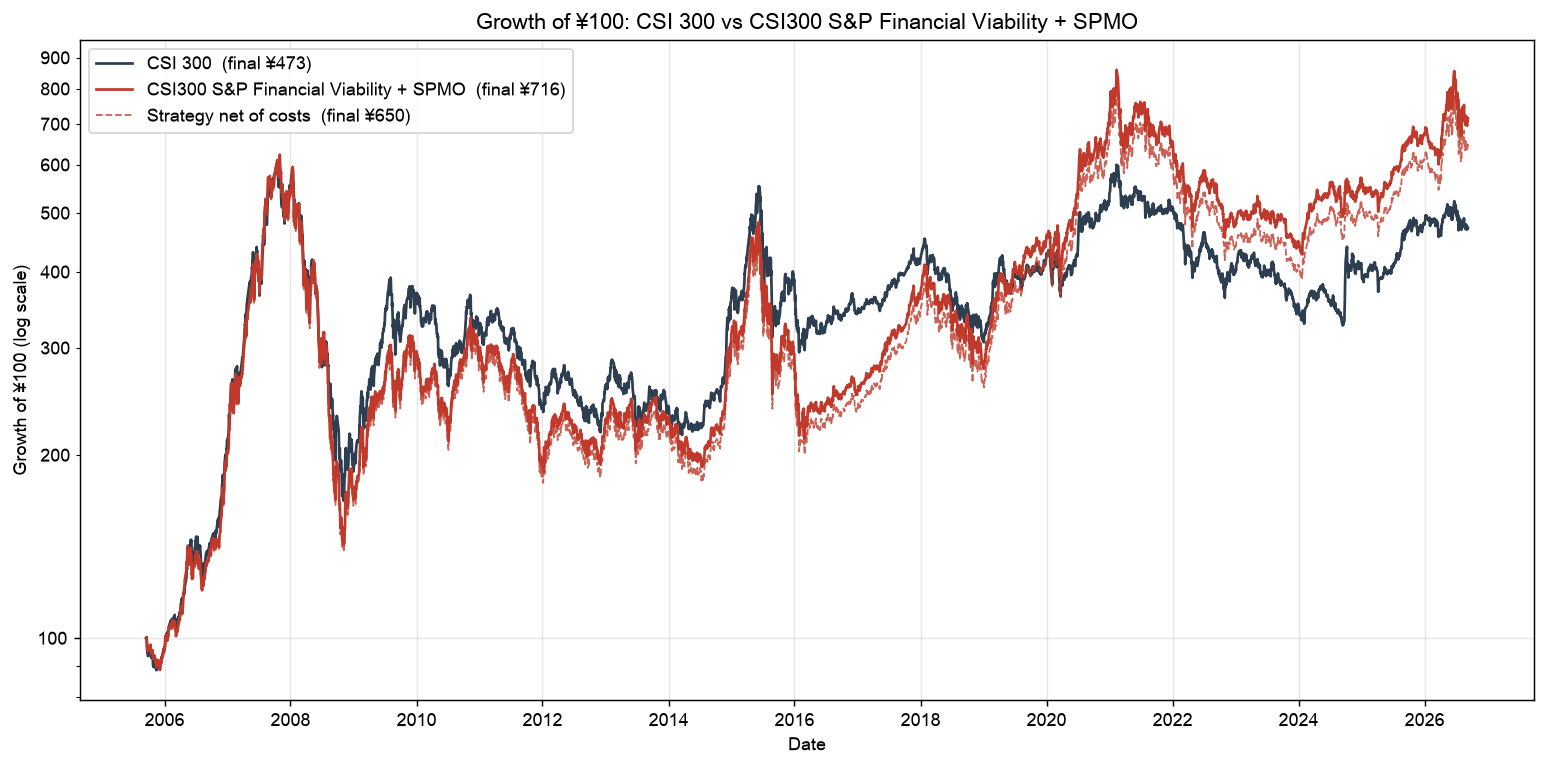
\includegraphics[width=\textwidth]{../charts/growth_of_100_log.png}
\caption{\textyen 100 的增长（对数坐标）：沪深300与本指数（费前 / 费后）}\label{fig:growth}
\end{figure}

\begin{figure}[!htbp]
\centering
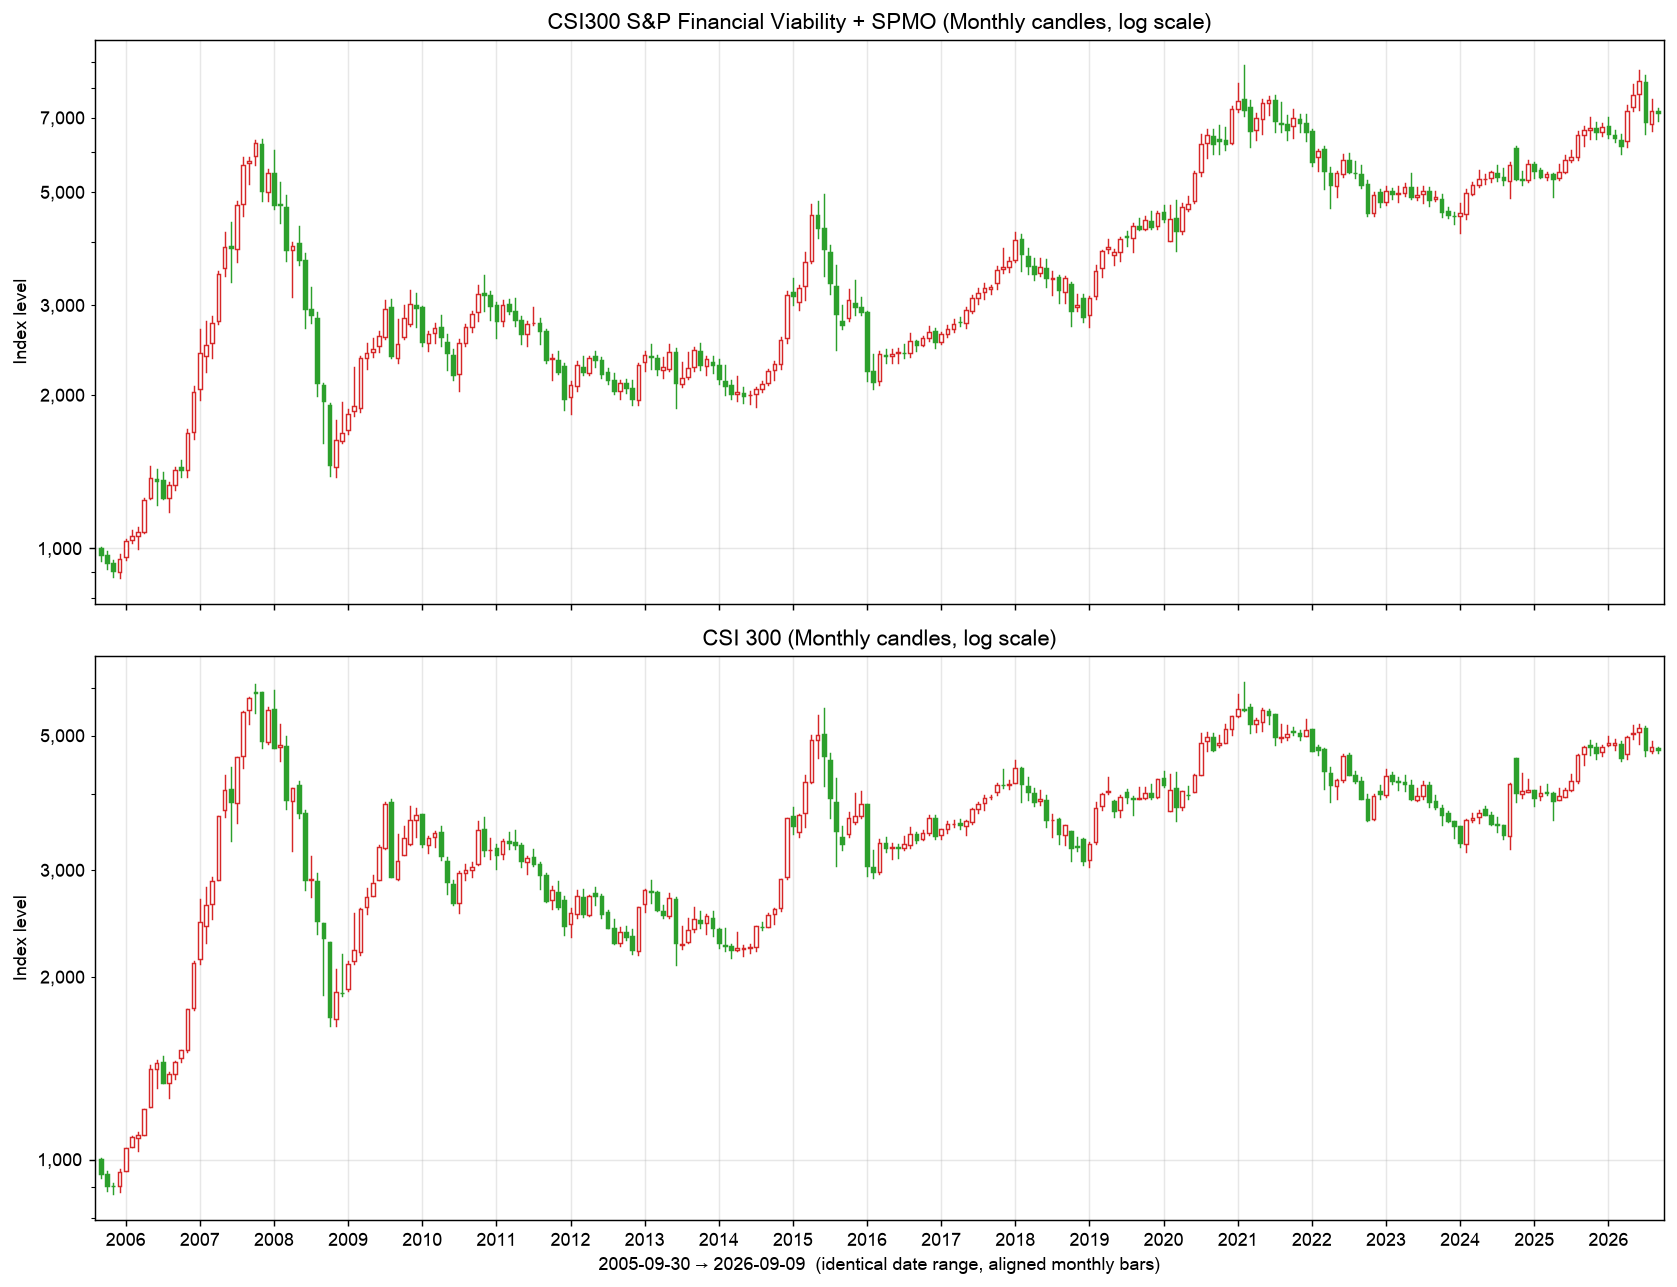
\includegraphics[width=\textwidth]{../charts/candlestick_comparison.png}
\caption{月 K 线比较：本指数（上）与沪深300（下），对数坐标，时间轴对齐}\label{fig:candles}
\end{figure}

\FloatBarrier
\subsection{年度收益}
\begin{table}[!htbp]
\centering
\footnotesize
\caption{日历年收益（2005 年自 9 月 16 日起，2026 年至 9 月 9 日止）}\label{tab:annual}
\begin{tabular}{@{}lrrrr@{}}
\toprule
年份 & 沪深300 & 策略 & 策略（费后） & 超额 \\
\midrule
2005 & $-$4.6\% & $-$4.8\% & $-$4.8\% & $-$0.2\% \\
2006 & +121.0\% & +113.0\% & +111.7\% & $-$8.0\% \\
2007 & +161.5\% & +168.5\% & +166.5\% & +6.9\% \\
2008 & $-$65.9\% & $-$69.0\% & $-$69.3\% & $-$3.1\% \\
2009 & +96.7\% & +75.5\% & +74.3\% & $-$21.2\% \\
2010 & $-$12.5\% & +0.8\% & +0.3\% & +13.3\% \\
2011 & $-$25.0\% & $-$34.2\% & $-$34.5\% & $-$9.1\% \\
2012 & +7.6\% & +16.5\% & +15.9\% & +9.0\% \\
2013 & $-$7.6\% & +0.0\% & $-$0.3\% & +7.7\% \\
2014 & +51.7\% & +37.3\% & +36.6\% & $-$14.4\% \\
2015 & +5.6\% & $-$7.5\% & $-$7.9\% & $-$13.1\% \\
2016 & $-$11.3\% & $-$12.9\% & $-$13.3\% & $-$1.6\% \\
2017 & +21.8\% & +44.4\% & +44.0\% & +22.7\% \\
2018 & $-$25.3\% & $-$22.3\% & $-$22.5\% & +3.1\% \\
2019 & +36.1\% & +59.5\% & +58.9\% & +23.4\% \\
2020 & +27.2\% & +60.2\% & +59.7\% & +33.0\% \\
2021 & $-$5.2\% & $-$10.0\% & $-$10.3\% & $-$4.8\% \\
2022 & $-$21.6\% & $-$27.0\% & $-$27.3\% & $-$5.4\% \\
2023 & $-$11.4\% & $-$6.0\% & $-$6.4\% & +5.4\% \\
2024 & +14.7\% & +26.4\% & +26.1\% & +11.7\% \\
2025 & +17.7\% & +18.2\% & +17.8\% & +0.5\% \\
2026 & $-$1.2\% & +6.5\% & +6.3\% & +7.8\% \\
\bottomrule
\end{tabular}
\end{table}

22 个日历年中策略跑赢 12 年。绝对收益最强：2007 年（+168.5\%）、2006 年（+113.0\%）、2009 年（+75.5\%）；最弱：2008 年（$-$69.0\%）、2011 年（$-$34.2\%）、2022 年（$-$27.0\%）。超额最大：2020 年（+33.0\%）、2019 年（+23.4\%）、2017 年（+22.7\%）；超额最差：2009 年（$-$21.2\%）、2014 年（$-$14.4\%）、2015 年（$-$13.1\%）。跑输年份集中在两类环境：由低动量的金融、周期大盘股主导的急涨（2009、2014 年，即动量反转），以及长周期趋势中断后的震荡（2011、2015--2016 年）。
\begin{figure}[!htbp]
\centering
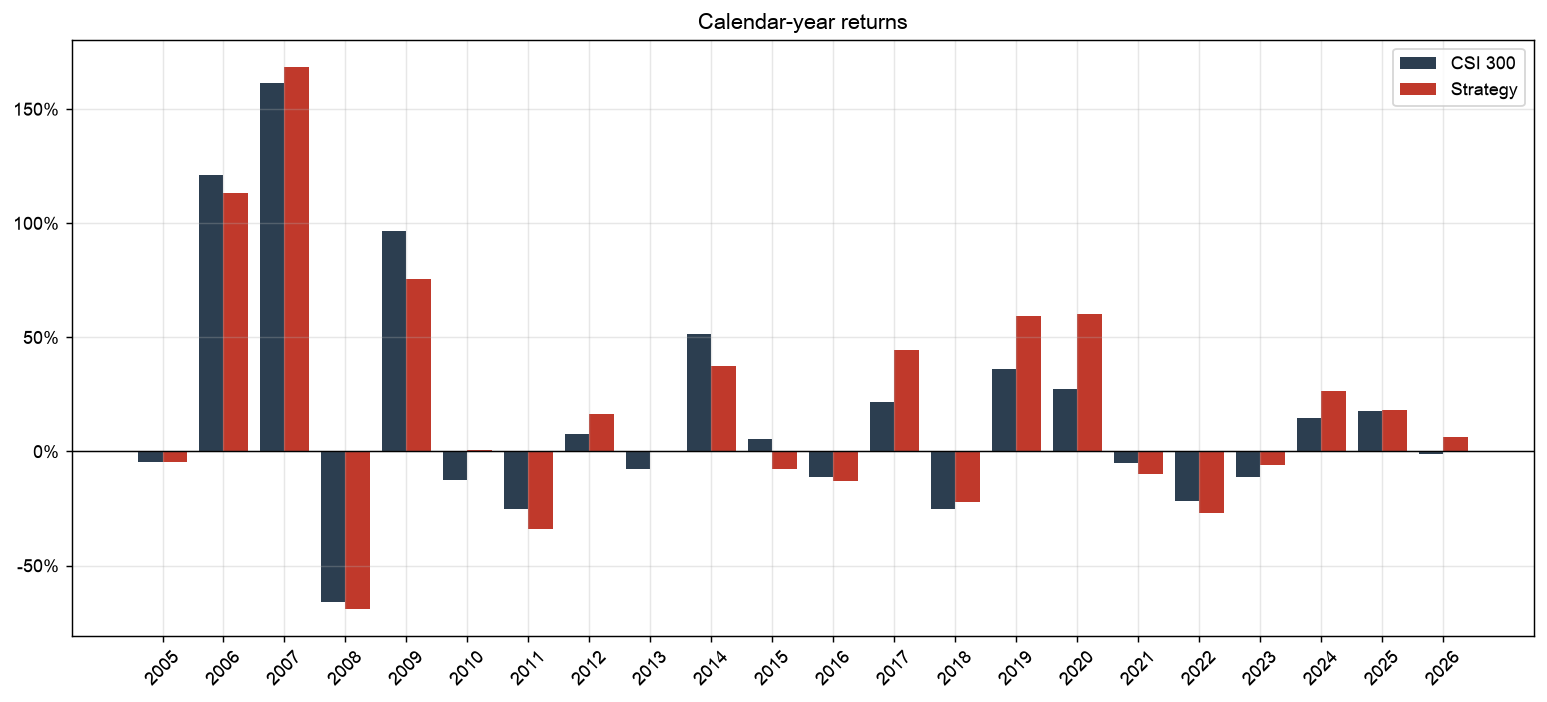
\includegraphics[width=0.9\textwidth]{../charts/annual_returns.png}
\caption{年度收益：沪深300与策略}\label{fig:annual}
\end{figure}

\FloatBarrier
\subsection{月度收益分布与上下行捕获}
\begin{table}[!htbp]
\centering
\small
\caption{月度收益分布（253 个月）}\label{tab:monthly}
\begin{tabular}{@{}lrr@{}}
\toprule
指标 & 沪深300 & 策略 \\
\midrule
月均收益 & 0.92\% & 1.13\% \\
月收益标准差 & 7.81\% & 8.30\% \\
偏度 & 0.08 & -0.08 \\
超额峭度 & 1.74 & 1.27 \\
正收益月份占比 & 56\% & 56\% \\
最佳月份 & 2007-04（+27.9\%） & 2007-04（+24.7\%） \\
最差月份 & 2008-10（$-$25.9\%） & 2008-08（$-$26.4\%） \\
\bottomrule
\end{tabular}
\end{table}

月度超额收益（策略减沪深300）均值 +0.21 个百分点、标准差 3.39 个百分点，为正的月份占 57\%，$t$ 统计量 0.97——在常规显著性水平下不能拒绝超额收益为零的假设。上行月份捕获比 1.04、下行月份捕获比 0.96；上涨月跑赢概率 55\%，下跌月跑赢概率 59\%；按日收益估计的上行 $\beta$ 0.95、下行 $\beta$ 1.00。策略在涨跌两种月份中的平均超额相近（+0.22 与 +0.19 个百分点），没有明显的方向性择时特征，超额主要来自个股选择（图 \ref{fig:monthly}）。
\begin{figure}[!htbp]
\centering
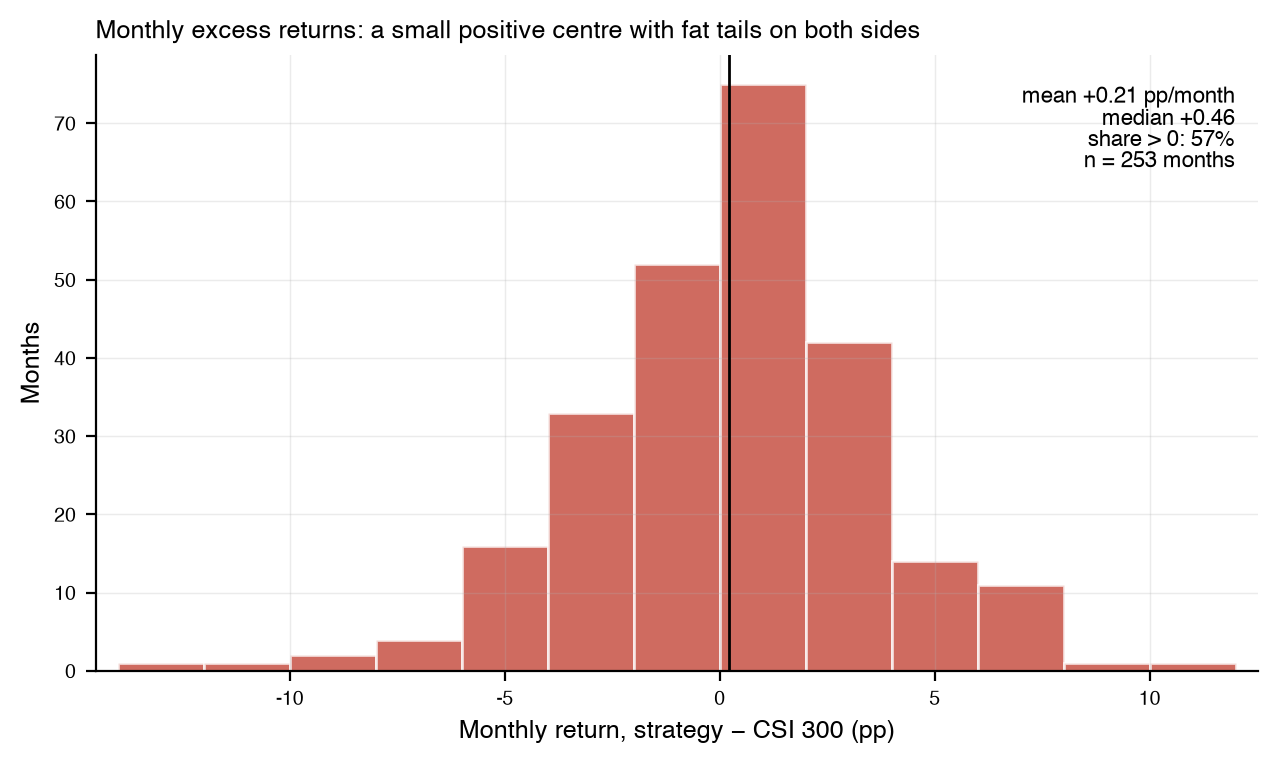
\includegraphics[width=0.85\textwidth]{../charts/research/rr_monthly_excess.png}
\caption{月度超额收益分布}\label{fig:monthly}
\end{figure}

\FloatBarrier
\subsection{回撤与尾部风险}
\begin{table}[!htbp]
\centering
\small
\caption{最大回撤（价格指数）}\label{tab:dd}
\begin{tabular}{@{}lrr@{}}
\toprule
指标 & 沪深300 & 策略 \\
\midrule
最大回撤 & $-$72.30\% & $-$77.16\% \\
峰值日期 & 2007-10-16 & 2007-10-31 \\
谷底日期 & 2008-11-04 & 2008-11-04 \\
恢复日期 & 尚未恢复 & 2020-07-13 \\
下跌天数 & 385 & 370 \\
恢复天数 & --- & 4269 \\
\bottomrule
\end{tabular}
\end{table}

\begin{table}[!htbp]
\centering
\footnotesize
\caption{日收益尾部统计（历史 VaR / CVaR）}\label{tab:tails}
\resizebox{\linewidth}{!}{%
\begin{tabular}{@{}lrrrrrrrrrrr@{}}
\toprule
系列 & 日均收益 & 日波动 & 偏度 & 超额峭度 & VaR 95\% & CVaR 95\% & VaR 99\% & CVaR 99\% & 最差单日 & $<-5\%$ 天数 & $>+5\%$ 天数 \\
\midrule
沪深300 & 0.043\% & 1.58\% & $-$0.38 & 4.41 & $-$2.39\% & $-$3.96\% & $-$4.95\% & $-$6.41\% & $-$9.24\% & 49 & 24 \\
策略 & 0.053\% & 1.71\% & $-$0.36 & 3.15 & $-$2.76\% & $-$4.24\% & $-$5.15\% & $-$6.57\% & $-$9.48\% & 57 & 27 \\
\bottomrule
\end{tabular}
}
\end{table}

两个指数在 2007--2008 年都经历了 70\% 以上的回撤，策略更深（$-$77.16\% 对 $-$72.30\%）；策略价格指数于 2020-07-13 收复 2007 年高点，而沪深300价格指数至今未收复。日收益尾部（VaR、CVaR、极端日数量）策略略重于沪深300，与其更高的波动一致。相对强度（策略 / 沪深300）的最大回撤为 $-$33.2\%，自 2007-08-09 持续至 2016-03-04，于 2019-08-16 才收复——\textbf{连续八年半跑输}是持有这类策略必须接受的代价（图 \ref{fig:dd}、图 \ref{fig:rs}）。
\begin{figure}[!htbp]
\centering
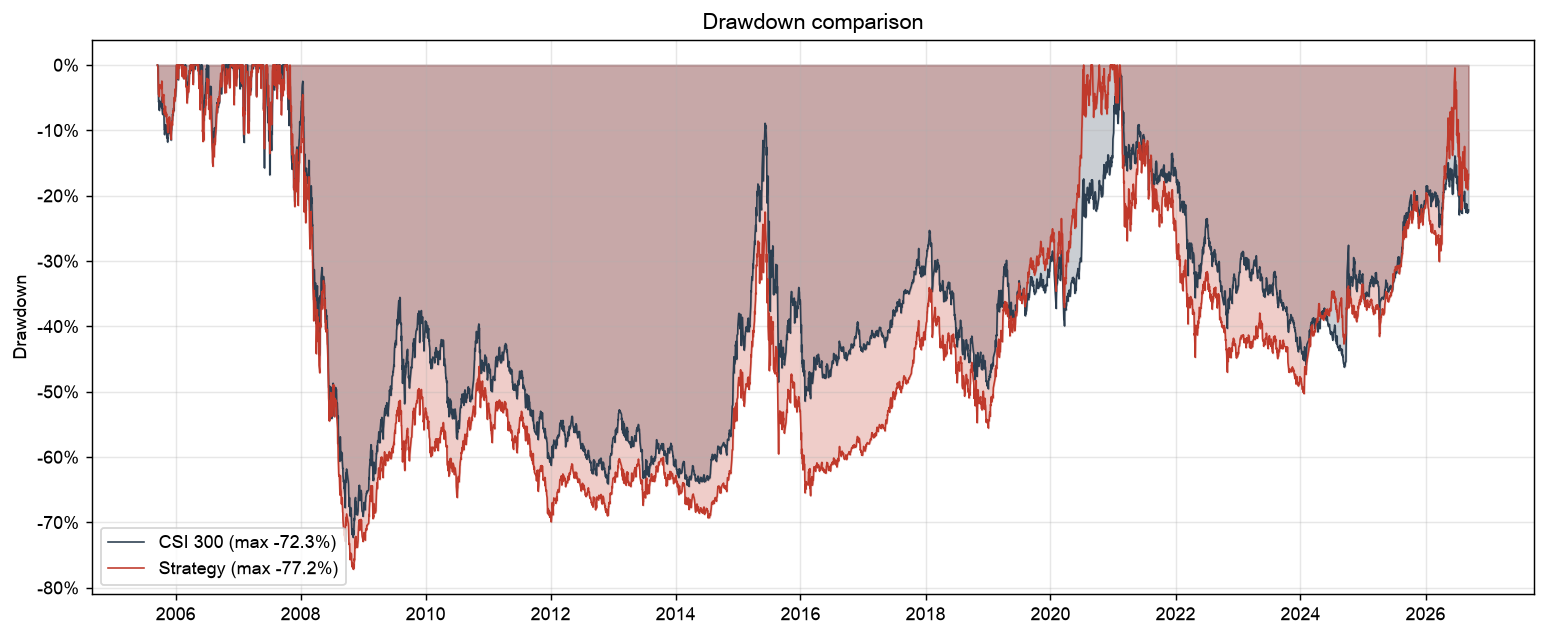
\includegraphics[width=\textwidth]{../charts/drawdown_comparison.png}
\caption{回撤比较}\label{fig:dd}
\end{figure}

\FloatBarrier
\subsection{滚动指标}
1 年滚动收益跑赢沪深300的比例 56.4\%（中位数超额 +2.1\%）；3 年滚动年化胜率 60.4\%（中位数 +1.7\%）；5 年滚动年化胜率 61.4\%（中位数 +1.4\%）。1 年滚动 $\beta$ 均值 0.98（0.45--1.41），滚动跟踪误差 5.6\%--17.9\%（均值 10.3\%），滚动信息比率中位数 0.26（图 \ref{fig:rolling}）。
\begin{figure}[!htbp]
\centering
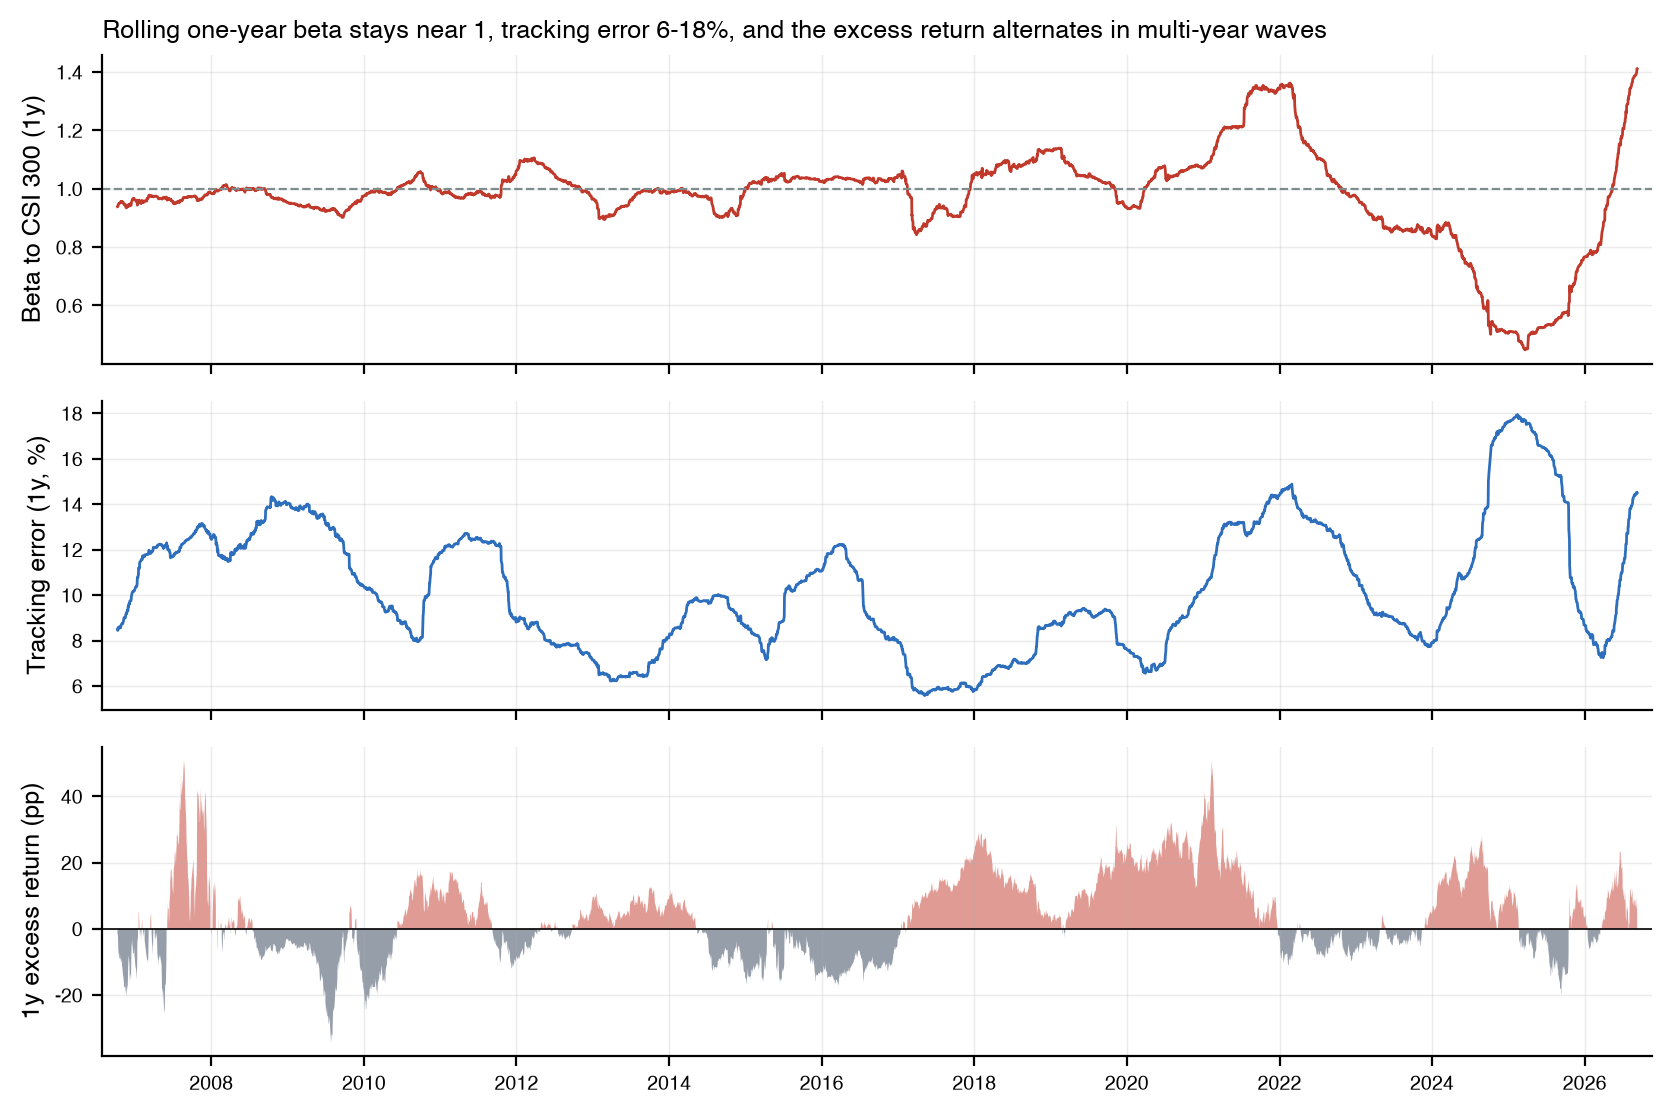
\includegraphics[width=\textwidth]{../charts/research/rr_rolling_beta_te.png}
\caption{滚动 1 年 $\beta$、跟踪误差与超额收益}\label{fig:rolling}
\end{figure}

\begin{figure}[!htbp]
\centering
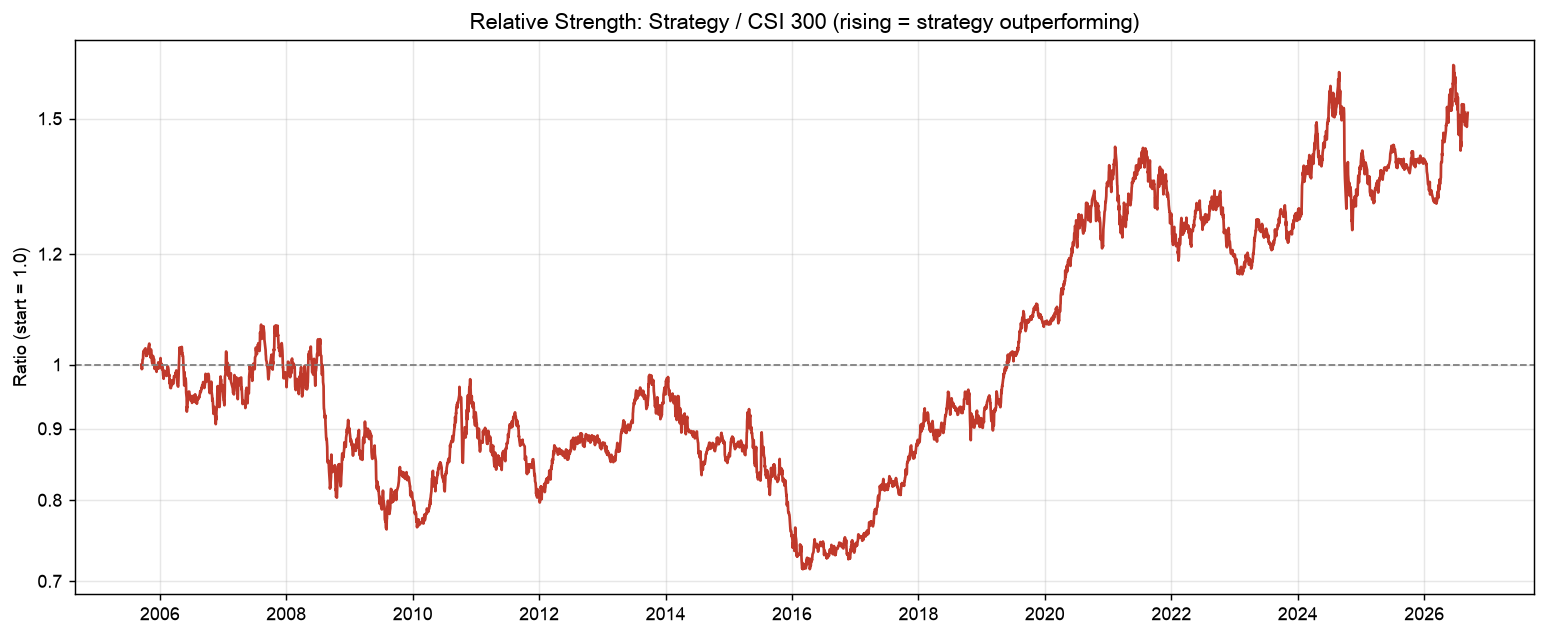
\includegraphics[width=0.9\textwidth]{../charts/relative_strength.png}
\caption{相对强度：策略 / 沪深300}\label{fig:rs}
\end{figure}

\FloatBarrier
\subsection{市场周期分析}
\begin{table}[!htbp]
\centering
\footnotesize
\caption{各市场阶段的表现（价格指数、费前）}\label{tab:cycles}
\resizebox{\linewidth}{!}{%
\begin{tabular}{@{}lrrrrrrrrrrr@{}}
\toprule
阶段 & 沪深300 & 策略 & 超额 & 沪深300年化 & 策略年化 & 沪深300波动 & 策略波动 & Sharpe (300) & Sharpe (策略) & 回撤 (300) & 回撤 (策略) \\
\midrule
2005-2007 & 451.8\% & 444.7\% & $-$7.1\% & 111.5\% & 110.3\% & 28.5\% & 29.8\% & 2.79 & 2.66 & $-$20.9\% & $-$21.7\% \\
2008 & $-$66.2\% & $-$69.0\% & $-$2.8\% & $-$66.4\% & $-$69.2\% & 47.8\% & 47.5\% & $-$2.02 & $-$2.21 & $-$71.6\% & $-$76.1\% \\
2009-2014 & 87.7\% & 82.2\% & $-$5.5\% & 11.1\% & 10.5\% & 23.5\% & 25.0\% & 0.57 & 0.53 & $-$44.9\% & $-$44.2\% \\
2015-2016 & $-$9.1\% & $-$22.0\% & $-$12.9\% & $-$4.7\% & $-$11.8\% & 31.4\% & 33.7\% & 0.01 & $-$0.20 & $-$46.7\% & $-$56.0\% \\
2017-2018 & $-$9.9\% & 11.3\% & +21.2\% & $-$5.1\% & 5.5\% & 16.5\% & 19.8\% & $-$0.23 & 0.37 & $-$31.9\% & $-$31.4\% \\
2019-2020 & 75.5\% & 159.5\% & +84.0\% & 32.5\% & 61.2\% & 21.0\% & 23.1\% & 1.45 & 2.19 & $-$16.1\% & $-$17.8\% \\
2021-2024 & $-$25.3\% & $-$23.0\% & +2.3\% & $-$7.1\% & $-$6.3\% & 18.4\% & 21.0\% & $-$0.31 & $-$0.21 & $-$45.6\% & $-$50.3\% \\
2025-latest & 19.7\% & 28.8\% & +9.1\% & 11.3\% & 16.2\% & 16.6\% & 23.3\% & 0.73 & 0.76 & $-$10.5\% & $-$21.8\% \\
\bottomrule
\end{tabular}
}
\end{table}

策略跑赢的阶段：2017-2018、2019-2020、2021-2024、2025-latest；跑输的阶段：2005-2007、2008、2009-2014、2015-2016（表 \ref{tab:cycles}、图 \ref{fig:cycle}）。规律与动量文献一致：\textbf{趋势延续、龙头持续领涨的结构性行情}（2017--2018 年的核心资产、2019--2020 年的消费、新能源与医药成长股）对策略最有利；\textbf{由估值修复和政策刺激触发的 V 型反转}（2009 年上半年、2014 年四季度、2024 年 9 月）以及\textbf{趋势反复的震荡市}（2011--2013、2015--2016 年）最不利。2005--2007 年大牛市中策略与指数几乎同步——那一轮领涨的正是权重最大的金融与周期股。
\begin{figure}[!htbp]
\centering
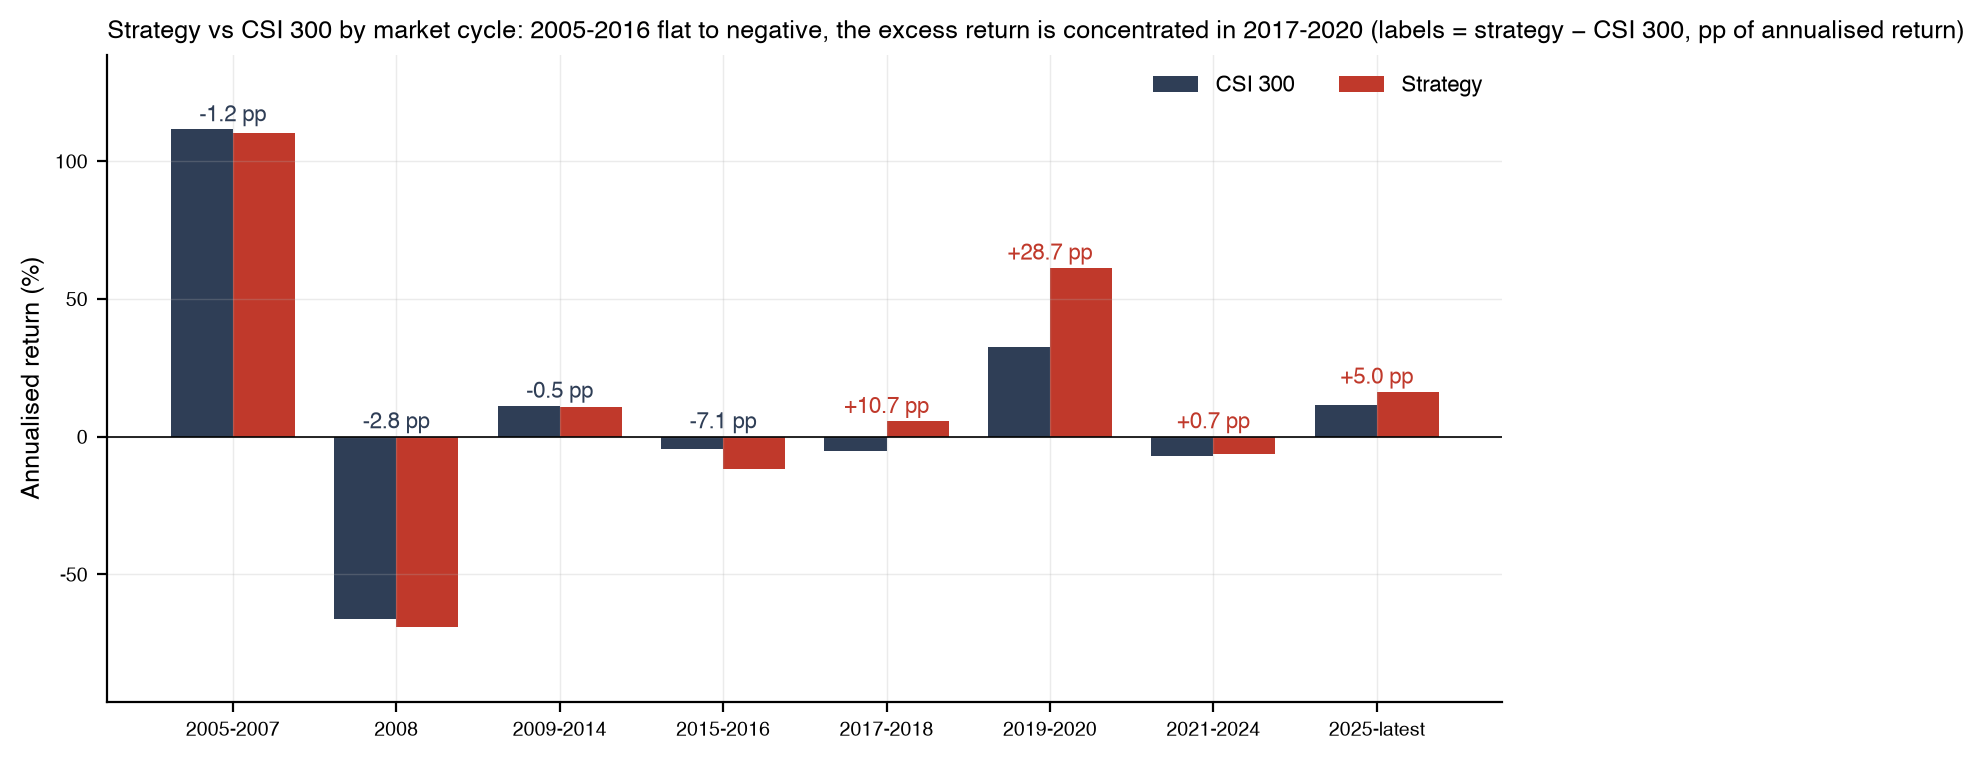
\includegraphics[width=\textwidth]{../charts/research/rr_cycle_cagr.png}
\caption{各市场阶段的年化收益（标签为策略减沪深300，单位：年化收益率的百分点）}\label{fig:cycle}
\end{figure}

\FloatBarrier
\subsection{动量崩塌}
\begin{table}[!htbp]
\centering
\small
\caption{最大的五次三个月相对回撤}\label{tab:crash}
\begin{tabular}{@{}llrrr@{}}
\toprule
结束日 & 开始日 & 策略 3 个月 & 沪深300 3 个月 & 相对 \\
\midrule
2024-12-03 & 2024-08-27 & $-$3.1\% & +19.6\% & $-$22.7\% \\
2009-07-31 & 2009-04-30 & +21.8\% & +42.4\% & $-$20.6\% \\
2008-10-20 & 2008-07-15 & $-$48.8\% & $-$33.5\% & $-$15.3\% \\
2022-02-11 & 2021-11-08 & $-$17.8\% & $-$5.1\% & $-$12.7\% \\
2023-01-30 & 2022-10-25 & +3.8\% & +15.8\% & $-$12.0\% \\
\bottomrule
\end{tabular}
\end{table}

5 次最大的三个月相对回撤中，3 次发生在\textbf{市场上涨}而非下跌中（2024-12、2009-07、2023-01），符合 \citet{daniel2016} 对动量崩塌的刻画：在高波动的熊市底部反弹时，此前被抛弃的低动量股票反弹最猛，而动量组合恰好低配它们。2024-08-27 至 2024-12-03 的一次相对 $-$22.7\% 是全样本最大的一次：2024 年 9 月 24 日一揽子政策出台后沪深300三个月上涨 19.6\%，而 3 月和 9 月两次调仓所持的高动量股（以周期资源、电子为主）合计 $-$3.1\%。半年一次的调仓频率意味着策略直到 2025 年 3 月才转向。
\section{组合特征}\label{sec:portfolio}
\FloatBarrier
\subsection{Financial Viability 筛选漏斗}
每个参考日 300 只成分股中平均 37 只（19--76 只）未通过财务资格，通过者 263 只（224--281）。不合格原因见表 \ref{tab:funnel} 与图 \ref{fig:funnel}。动量数据不足（新上市或长期停牌，窗口内交易日少于 150）平均每期再剔除 6.3 只。$Z$ 分数被 $\pm 3$ 截断的股票平均每期 2.6 只；入选门槛 Momentum Score 的中位数为 1.60（即 $Z \approx +0.60$），最高分中位数 4.00。
\begin{table}[!htbp]
\centering
\small
\caption{Financial Viability 不合格原因合计（43 个参考日）}\label{tab:funnel}
\begin{tabular}{@{}lrr@{}}
\toprule
不合格原因 & 股票 $\times$ 期次 & 占比 \\
\midrule
无财务报表（多为已退市公司） & 535 & 34.1\% \\
最近一季 $\leq 0$ 且最近四季合计 $\leq 0$ & 379 & 24.1\% \\
仅最近一季 $\leq 0$ & 321 & 20.4\% \\
仅最近四季合计 $\leq 0$ & 279 & 17.8\% \\
仅 3 个连续季度已公布 & 31 & 2.0\% \\
仅 2 个连续季度已公布 & 12 & 0.8\% \\
仅 1 个季度已公布 & 8 & 0.5\% \\
参考日前无任何已公布报表 & 5 & 0.3\% \\
\bottomrule
\end{tabular}
\end{table}

\begin{figure}[!htbp]
\centering
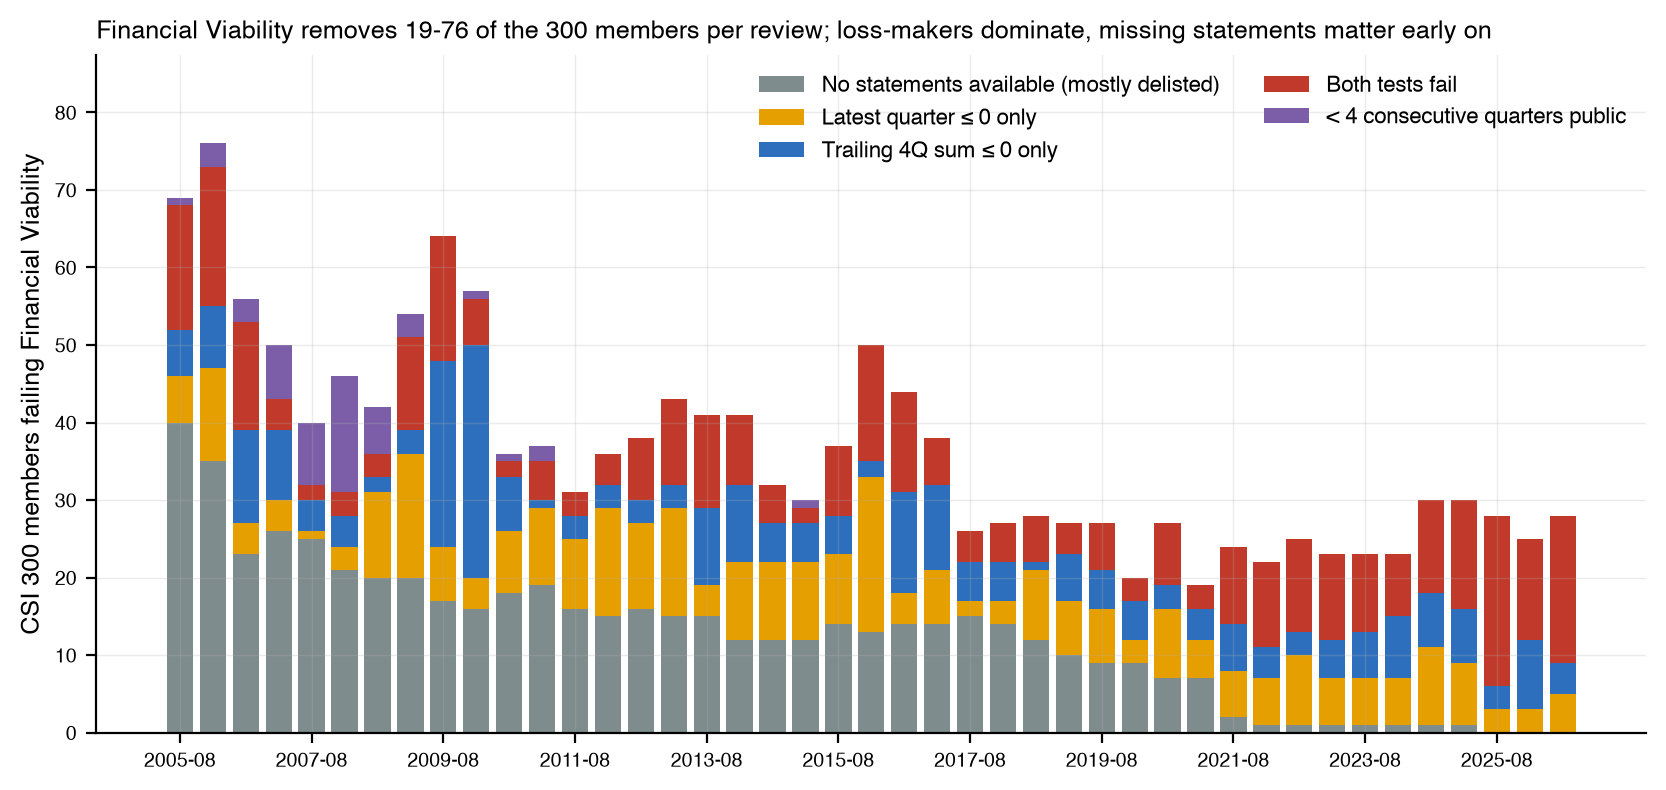
\includegraphics[width=\textwidth]{../charts/research/rr_fv_funnel.png}
\caption{各参考日未通过 Financial Viability 的成分股数量及原因}\label{fig:funnel}
\end{figure}

\FloatBarrier
\subsection{成分数量、集中度与权重上限}
成分股数量 45--55 只（均值 51.3）；有效成分数 $1/\sum_i w_i^2$ 为 19--37（均值 25.3），即权重集中度大约相当于一个 25 只的等权组合。前十大权重合计均值 53\%（38\%--65\%）；最大单一权重均值 8.9\%，9\% 上限平均每期约束 1.9 只。策略持有的股票合计占沪深300（代理）市值的 24\%（11\%--42\%）；策略权重落在沪深300市值前 100 名股票上的比例均值 81\%，即策略整体仍是大盘股组合，但相对母指数明显向中等市值倾斜（图 \ref{fig:conc}）。入选股票 Momentum Score 均值 2.50，最低入选分数均值 1.62。
\begin{figure}[!htbp]
\centering
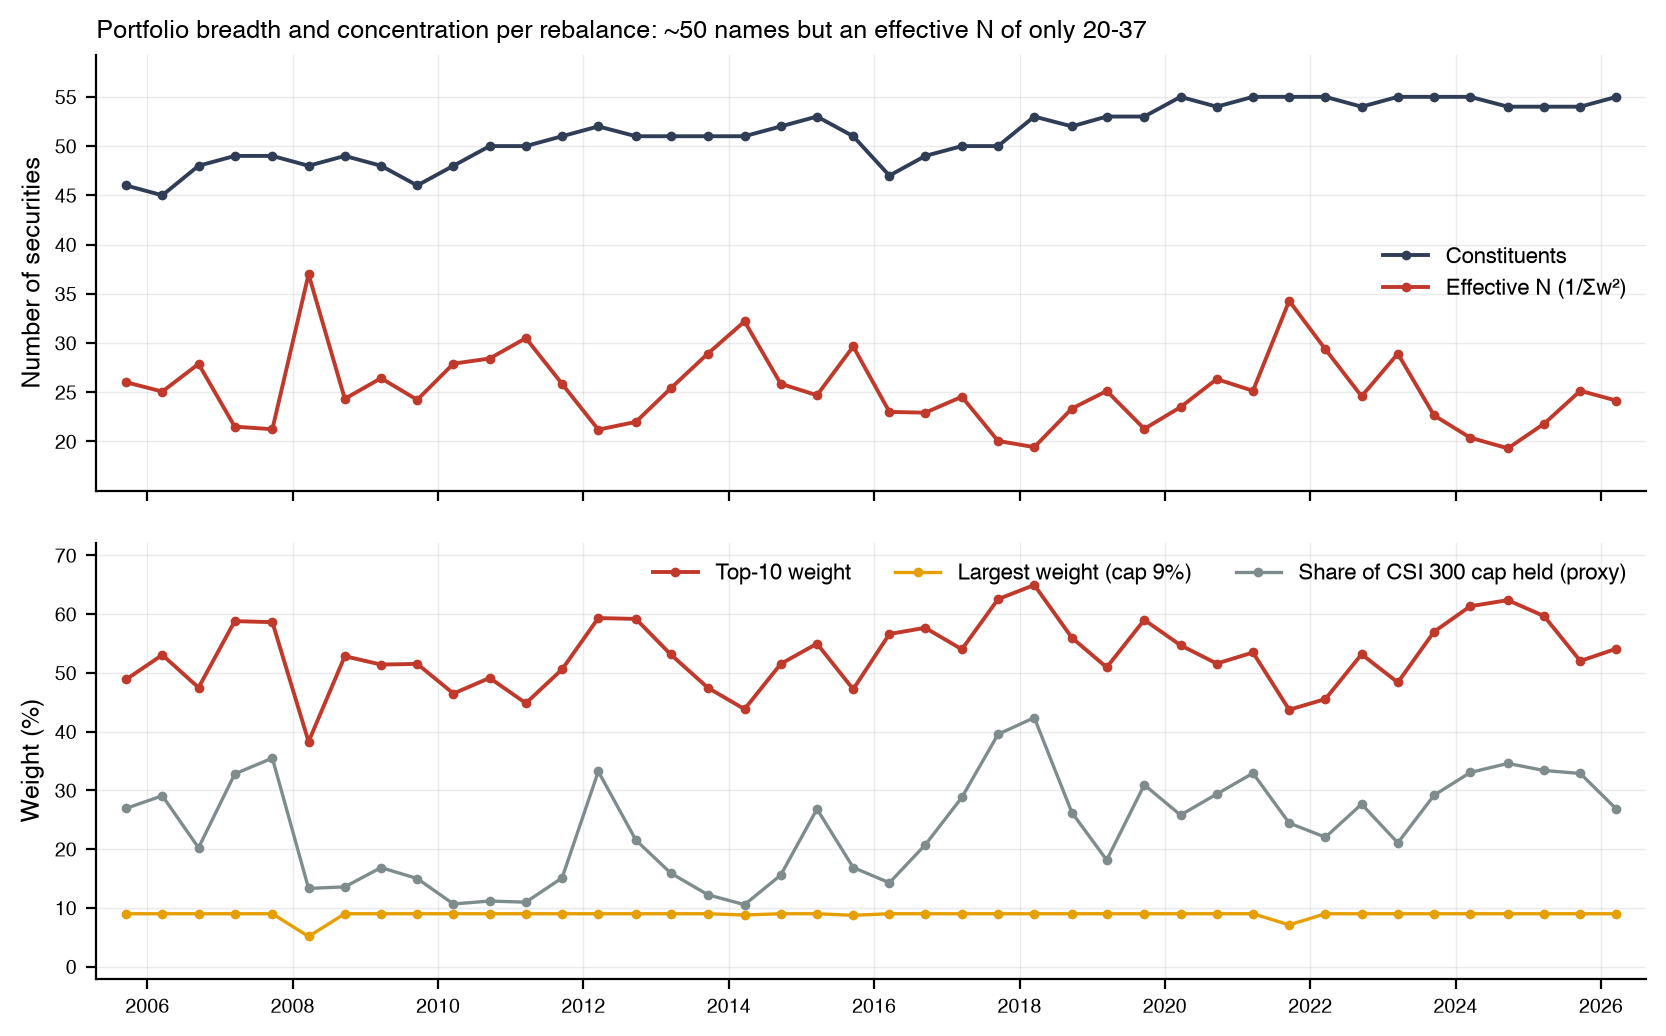
\includegraphics[width=\textwidth]{../charts/research/rr_concentration.png}
\caption{每次调仓的成分数量、有效成分数与集中度}\label{fig:conc}
\end{figure}

\FloatBarrier
\subsection{成分持续性与换手}
42 次已实施调仓共出现过 547 只不同的成分股。相邻两期成分股的平均保留率 45\%；一段连续成员期的平均长度 1.8 期（中位数 1 期），51\% 的成员期只持续一次调仓——动量组合的“短记忆”特征（图 \ref{fig:pers}）。入选次数最多的股票：贵州茅台（20 次）、五粮液（17 次）、恒瑞医药（16 次）、山东黄金（15 次）、泸州老窖（15 次）、同仁堂（14 次）、招商银行（14 次）、三一重工（14 次）、格力电器（14 次）、福耀玻璃（14 次）。单边换手每次调仓平均 55.1\%（最高 82.8\%），折合每年 107.7\%，与 S\&P 500 Momentum 公布的换手水平相当。
\begin{figure}[!htbp]
\centering
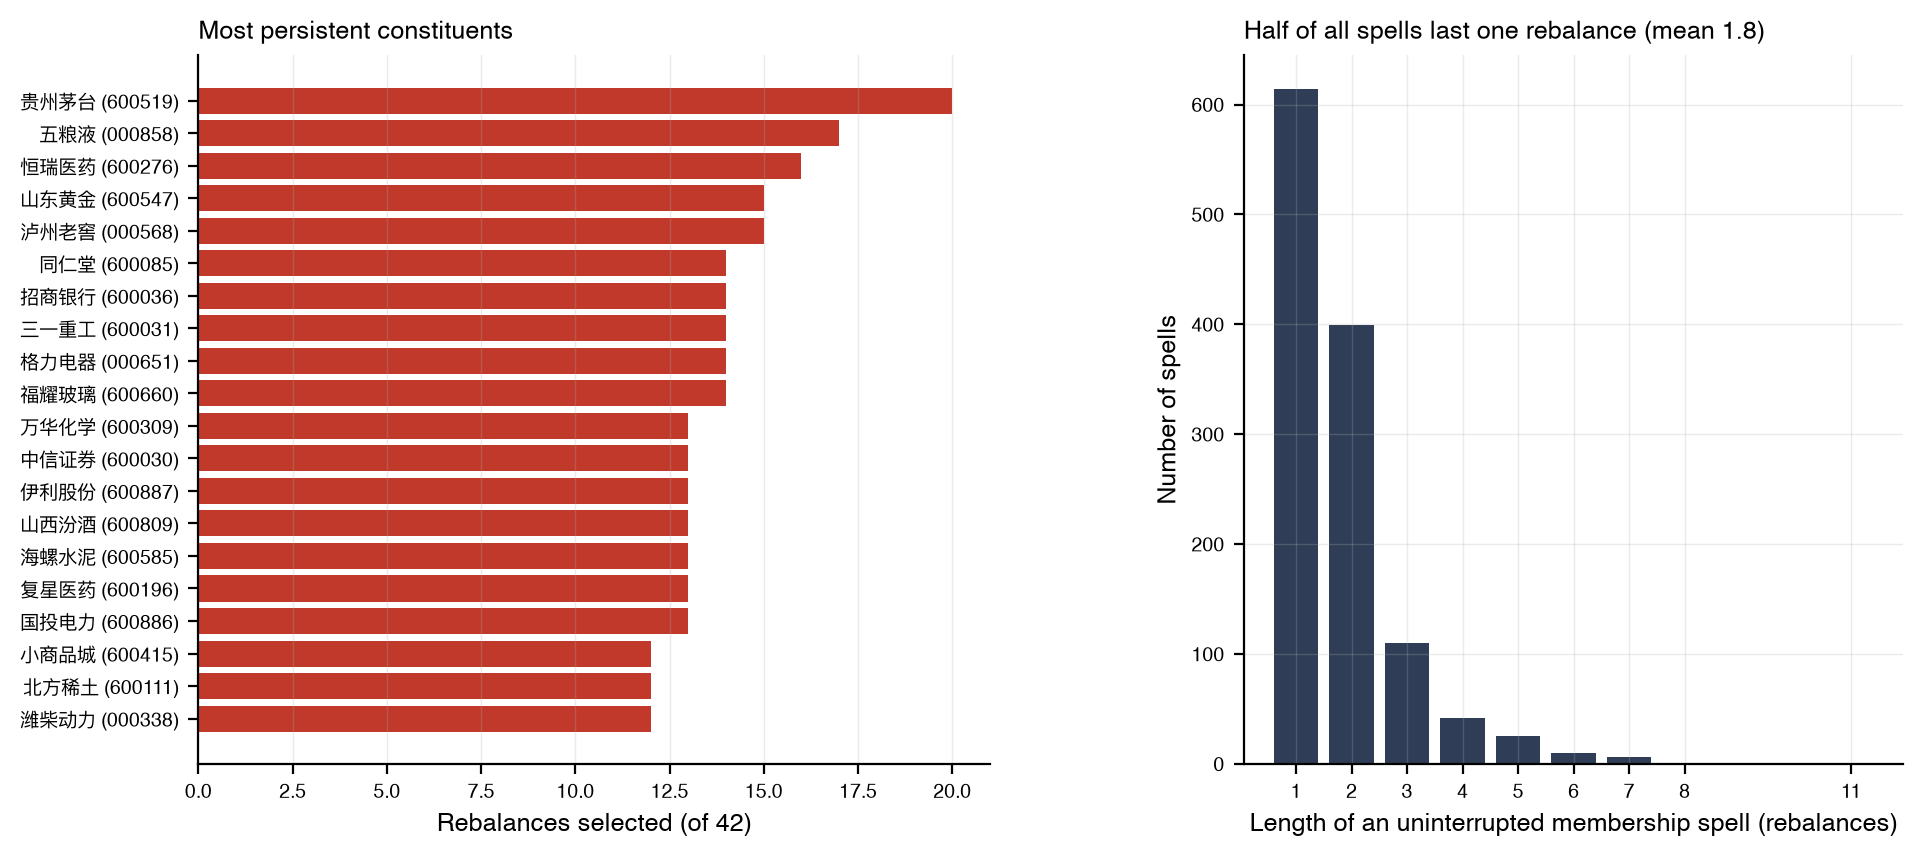
\includegraphics[width=\textwidth]{../charts/research/rr_persistence.png}
\caption{成分股持续性：入选次数最多的股票（左）与连续成员期长度分布（右）}\label{fig:pers}
\end{figure}

\FloatBarrier
\subsection{行业暴露（当前分类）}
历史行业分类没有免费的点位数据，此处只用中证沪深300一级行业指数的\emph{当前}成分对\emph{最新两期}名单分类（表 \ref{tab:sector}、图 \ref{fig:sector}）。
\begin{table}[!htbp]
\centering
\small
\caption{行业暴露：沪深300官方权重与最新两期策略名单}\label{tab:sector}
\begin{tabular}{@{}lrrr@{}}
\toprule
中证一级行业 & 沪深300 (2026-08-31) & 策略 2026-03-20 & 策略 2026-09-18 （待实施） \\
\midrule
信息技术 & 22.6\% & 30.2\% & 45.3\% \\
金融 & 19.9\% & 13.5\% & 0.0\% \\
工业 & 16.2\% & 8.5\% & 15.0\% \\
通信服务 & 9.9\% & 13.8\% & 16.7\% \\
原材料 & 9.6\% & 32.7\% & 15.9\% \\
主要消费 & 6.4\% & 0.0\% & 0.0\% \\
可选消费 & 5.4\% & 0.0\% & 3.4\% \\
医药卫生 & 4.3\% & 1.3\% & 2.0\% \\
公用事业 & 2.8\% & 0.0\% & 0.0\% \\
能源 & 2.7\% & 0.0\% & 1.8\% \\
房地产 & 0.3\% & 0.0\% & 0.0\% \\
\bottomrule
\end{tabular}
\end{table}

相对沪深300，最新已实施名单最高配原材料（$+$23.1 个百分点）和信息技术（$+$7.6），最低配工业（$-$7.7）和主要消费（$-$6.4）。SPMO 类规则不做行业中性，行业暴露随动量所在板块大幅摆动，这是其超额收益与跟踪误差的共同来源。
\begin{figure}[!htbp]
\centering
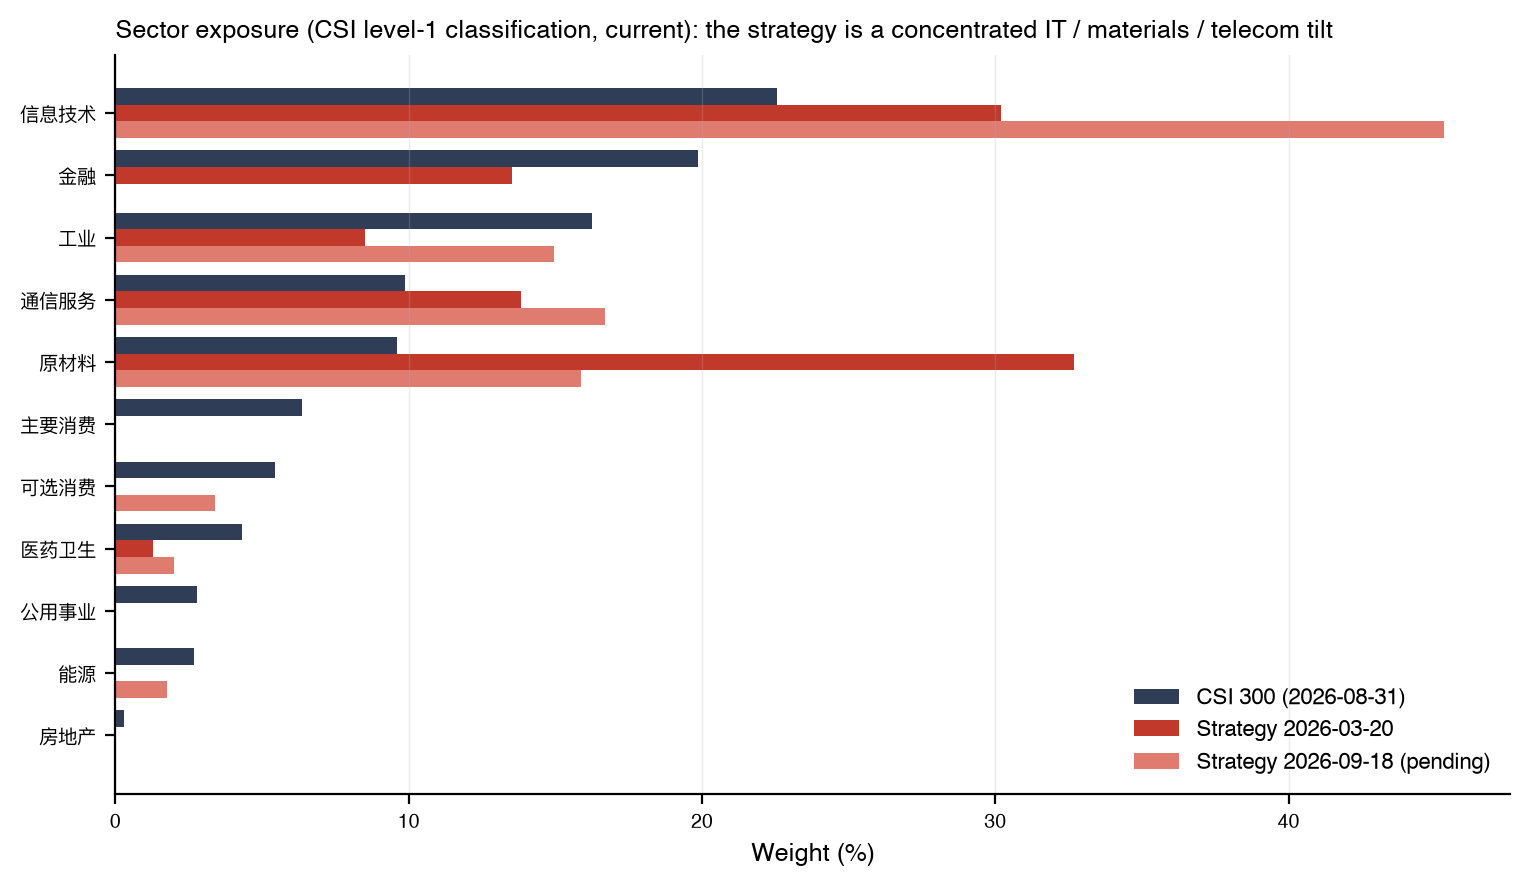
\includegraphics[width=0.9\textwidth]{../charts/research/rr_sector_exposure.png}
\caption{行业暴露：沪深300与最新两期名单（当前中证一级行业分类）}\label{fig:sector}
\end{figure}

最新持仓与待实施名单见附录 \ref{app:holdings}。
\section{收益来源分解：选股还是加权？}\label{sec:attribution}
用同一指数引擎、同样的调仓日期与成分股名单，只改变权重方案，可以把策略相对母指数的超额拆开（价格指数、费前；表 \ref{tab:attr}、图 \ref{fig:attr}）。
\begin{table}[!htbp]
\centering
\small
\caption{同一批成分股在不同权重方案下的表现}\label{tab:attr}
\begin{tabular}{@{}p{6.4cm}rrp{4.6cm}@{}}
\toprule
组合 & \textyen 100 终值 & 年化 & 含义 \\
\midrule
沪深300（官方） & \textyen472.6 & 7.68\% & --- \\
沪深300复制（全部成分股，本文权重代理，同日期调仓） & \textyen381.5 & 6.59\% & 权重代理相对官方指数的偏差 \\
入选成分股，按自由流通市值（代理）加权 & \textyen697.4 & 9.70\% & 选股效应（相对复制指数） \\
入选成分股，SPMO 加权（本指数） & \textyen715.6 & 9.83\% & Momentum Score 倾斜与上限（相对市值加权） \\
入选成分股，等权 & \textyen762.9 & 10.17\% & 参照：完全去除市值倾斜 \\
\bottomrule
\end{tabular}
\end{table}

\begin{itemize}
\item \textbf{选股效应}（同一权重口径下，前 20\% 动量股对全部 300 只）：$+$3.11 个百分点/年，是超额收益的主体。
\item \textbf{Momentum Score 加权倾斜}（相对同一篮子的市值加权）：$+$0.13 个百分点/年——SPMO 式加权在 A 股历史上带来的增益有限。
\item \textbf{等权对市值加权}：$+$0.47 个百分点/年，说明在入选篮子内部，市值越大的股票（多为国有大盘股）动量延续性越差。
\item \textbf{权重代理偏差}：-1.09 个百分点/年。代理高配国有大盘股，用它复制沪深300会跑输官方指数；策略权重同样受此影响，因此策略相对官方沪深300 $+$2.15 个百分点的年化超额很可能低于真实自由流通加权版本能取得的水平。
\end{itemize}
\begin{figure}[!htbp]
\centering
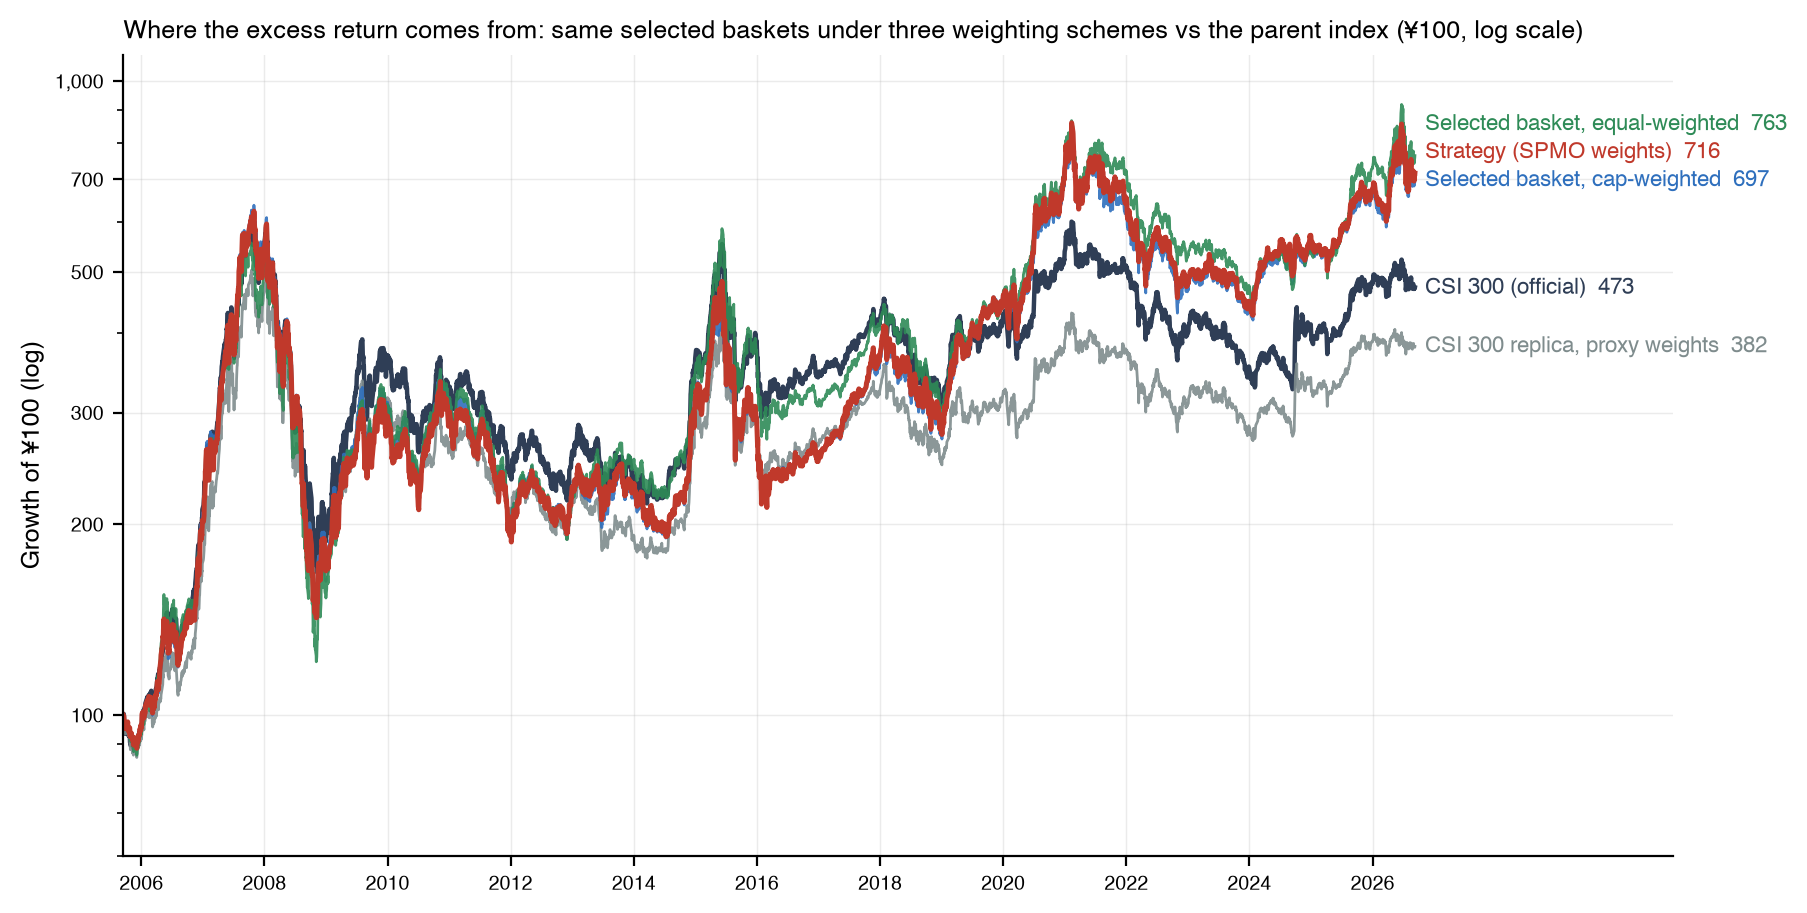
\includegraphics[width=\textwidth]{../charts/research/rr_attribution.png}
\caption{同一批成分股在三种权重方案下的表现，以及用权重代理复制的沪深300（\textyen 100，对数坐标）}\label{fig:attr}
\end{figure}

\section{交易成本与可实施性}\label{sec:cost}
费后指数按当期实际制度扣费：佣金随历史下调、印花税按各时期税率（2008 年 9 月起仅卖出征收、2023 年 8 月起减半）、过户费与固定冲击成本。费前年化 9.83\%，费后 9.33\%，年化成本拖累 0.50\%；21 年累计支付的成本相当于期末净值的 9.9\%。各年单边换手见表 \ref{tab:turnover}。成分股全部为沪深300成分、流动性充足，半年一次调仓、单边换手约 55\%，对资金规模不敏感；主要摩擦来自停牌股票（回测按停牌前价格成交）以及涨跌停板日无法足量成交。
\begin{table}[!htbp]
\centering
\small
\caption{各日历年的单边换手率}\label{tab:turnover}
\begin{tabular}{@{}lrlr@{}}
\toprule
年份 & 单边换手 & 年份  & 单边换手  \\
\midrule
2006 & 107\% & 2017 & 88\% \\
2007 & 100\% & 2018 & 72\% \\
2008 & 138\% & 2019 & 107\% \\
2009 & 141\% & 2020 & 84\% \\
2010 & 121\% & 2021 & 92\% \\
2011 & 115\% & 2022 & 121\% \\
2012 & 127\% & 2023 & 123\% \\
2013 & 97\% & 2024 & 71\% \\
2014 & 130\% & 2025 & 95\% \\
2015 & 123\% & 2026 & 65\% \\
2016 & 144\% &  &  \\
\bottomrule
\end{tabular}
\end{table}

\section{与 HSI300-Momentum-Strategy 的对比}\label{sec:hsmo}
GitHub 项目 HSI300-Momentum-Strategy \cite{hsmo} 同样受 SPMO 启发在沪深300内做动量选股，但设计取向不同：它是一个\textbf{集中持股的量化组合}（Top-20 等权、季度调仓、行业上限），而本文是一只\textbf{指数}（约 50 只、市值乘以分数加权、半年调仓、缓冲与上限）。本节先比较规则（表 \ref{tab:hsmo_rules}），再用本文的数据复现其规则，在相同窗口和相同数据上比较结果。
\begin{table}[!htbp]
\centering
\footnotesize
\caption{两个项目的规则差异}\label{tab:hsmo_rules}
\begin{tabular}{@{}p{1.9cm}p{6.2cm}p{6.6cm}@{}}
\toprule
项目 & HSI300-Momentum-Strategy & 本文 \\
\midrule
数据源 & BaoStock：每月末 hs300 成分快照、后复权收盘价、当前行业分类 & 中证公告逐日点位成分（2005 起）、新浪 / 东财原始价格自建复权、季度财报与公告日 \\
成分股口径 & 调仓日采用最近一个月末快照 & 调仓日当日有效成分；调仓期间被剔除的持仓同日剔除 \\
盈利筛选 & 无 & S\&P Financial Viability \\
动量信号 & $P_{t-22}/P_{t-253}-1$ 除以 252 日日收益标准差（窗口含最近一月），$T-1$ 计算 $T$ 交易 & 12--1 月价格变动除以同窗口日收益标准差；参考日计算，三周后实施 \\
标准化 / 分数 & 无（按原始风险调整动量排序） & 横截面 $Z$ 分数（$\pm 3$ 截断）→ Momentum Score \\
选样 & Top 20，每个（当前）行业最多 5 只 & 合格股票前 20\%（约 45--55 只），S\&P 20\% 缓冲，母指数资格优先 \\
权重 & 等权 & 自由流通市值 $\times$ Score，公司上限 $\min(9\%,\,20\,w^P)$ \\
调仓频率 & 季度（自然季末最后一个交易日收盘） & 半年（2 / 8 月末参考，3 / 9 月第三个星期五实施） \\
收益口径 & 策略用后复权价（含股息）对沪深300价格指数 & 价格指数与全收益指数分别对应比较 \\
成本 & 成交金额的 15\,bp（买卖同费率） & 按历史制度的佣金、印花税、过户费与冲击成本 \\
回测区间 & 2019-01-01 → 2025-12-20（7 年） & 2005-09-16 → 2026-09-09（21 年） \\
资格审计 & 无 & 每期自动审计成员资格、财报公告日、动量数据可得性 \\
\bottomrule
\end{tabular}
\end{table}

\FloatBarrier
\subsection{其公布结果与在本文数据上的复现（2019--2025）}
我们按其代码逐条复现规则（信号、季末调仓、等权、漂移、15\,bp 成本），只把数据换成本文的点位成分与复权价格。行业上限使用当前中证一级行业分类（其代码同样使用当前分类），历史上已不在沪深300的股票无分类，归入“未知”一类同样受 5 只上限约束。表 \ref{tab:hsmo_win} 与表 \ref{tab:hsmo_ann} 给出结果；其公布值转录自该仓库 README 中的结果图。
\begin{table}[!htbp]
\centering
\footnotesize
\caption{HSMO 仓库公布值与在本文数据上的复现，2019-01-01 至 2025-12-20；夏普比率按其代码以 2\% 无风险利率计算}\label{tab:hsmo_win}
\begin{tabular}{@{}lrrrrr@{}}
\toprule
系列 & 累计收益 & 年化收益 & 年化波动 & 夏普 (rf=2\%) & 最大回撤 \\
\midrule
HSMO 仓库公布值（策略） & 283.6\% & 22.2\% & 24.4\% & 0.83 & $-$33.5\% \\
HSMO 仓库公布值（沪深300） & 53.8\% & 6.6\% & 19.1\% & 0.24 & $-$45.6\% \\
复现：HSMO 规则，行业上限（当前分类） & 235.7\% & 19.8\% & 24.4\% & 0.73 & $-$39.7\% \\
复现：HSMO 规则，无行业上限 & 221.2\% & 19.0\% & 24.7\% & 0.69 & $-$41.0\% \\
复现：HSMO 规则，无上限，本项目成本模型 & 218.9\% & 18.9\% & 24.7\% & 0.68 & $-$41.1\% \\
本指数：全收益，费前 & 182.0\% & 16.7\% & 21.2\% & 0.69 & $-$46.4\% \\
本指数：全收益，费后 & 175.3\% & 16.3\% & 21.2\% & 0.68 & $-$47.0\% \\
本指数：价格，费前 & 135.8\% & 13.6\% & 21.2\% & 0.55 & $-$50.3\% \\
沪深300（价格） & 53.8\% & 6.6\% & 19.1\% & 0.24 & $-$45.6\% \\
沪深300（全收益） & 81.8\% & 9.3\% & 19.1\% & 0.38 & $-$41.6\% \\
\bottomrule
\end{tabular}
\end{table}

\begin{table}[!htbp]
\centering
\footnotesize
\caption{逐年收益：HSMO 公布值、复现值与本指数}\label{tab:hsmo_ann}
\resizebox{\linewidth}{!}{%
\begin{tabular}{@{}lrrrrrr@{}}
\toprule
年份 & 公布：策略 & 公布：沪深300 & 复现：行业上限 & 复现：无上限 & 本指数 TR 费后 & 沪深300（本文数据） \\
\midrule
2019 & 40.9\% & 38.0\% & 43.7\% & 43.2\% & 63.8\% & 38.0\% \\
2020 & 85.9\% & 27.2\% & 70.8\% & 71.3\% & 61.4\% & 27.2\% \\
2021 & 11.1\% & $-$5.2\% & 9.5\% & 7.0\% & $-$9.7\% & $-$5.2\% \\
2022 & $-$8.7\% & $-$21.6\% & $-$14.3\% & $-$13.9\% & $-$25.3\% & $-$21.6\% \\
2023 & $-$6.5\% & $-$11.4\% & $-$8.8\% & $-$7.0\% & $-$2.4\% & $-$11.4\% \\
2024 & 30.8\% & 14.7\% & 30.8\% & 30.4\% & 31.7\% & 14.7\% \\
2025 & 17.8\% & 16.1\% & 22.2\% & 17.2\% & 20.2\% & 16.1\% \\
\bottomrule
\end{tabular}
}
\end{table}

复现结果与其公布值方向一致、量级接近：沪深300年度收益逐年完全相同（两边都用官方价格指数），策略年化 19.8\% 对公布的 22.2\%，差异主要来自 2020 年（复现 70.8\% 对公布 85.9\%）和 2022 年，源于成分股快照口径（月末快照对逐日）、复权价格与行业分类的差别，而非规则本身。因此可以把两条曲线放在同一数据上比较：2019--2025 年 HSMO 规则 \textyen 100 → \textyen321（无行业上限）/ \textyen335（行业上限），本指数全收益费后 \textyen275，沪深300全收益 \textyen182。HSMO 规则在这 7 年里收益更高、最大回撤更小（$-$41.0\% 对本指数全收益 $-$47.0\%）——差别主要在 2021--2022 年：季度调仓的等权组合在 2021 年 2 月核心资产见顶后一个季度内就转向，而半年调仓的本指数持有 2 月底确定的名单直到 9 月。
\FloatBarrier
\subsection{全样本、同数据比较（2005--2026）}
\begin{table}[!htbp]
\centering
\footnotesize
\caption{2005-09-16 至 2026-09-09，两套规则在同一数据上的表现}\label{tab:hsmo_full}
\begin{tabular}{@{}lrrrrr@{}}
\toprule
系列 & 累计收益 & 年化收益 & 年化波动 & 夏普 (rf=2\%) & 最大回撤 \\
\midrule
复现：HSMO 规则，无行业上限，15\,bp & 1114.8\% & 13.1\% & 28.9\% & 0.39 & $-$73.7\% \\
复现：HSMO 规则，无上限，本项目成本模型 & 1047.6\% & 12.8\% & 28.9\% & 0.37 & $-$73.9\% \\
复现：HSMO 规则，行业上限（当前分类） & 2122.3\% & 16.6\% & 28.1\% & 0.52 & $-$71.0\% \\
本指数：全收益，费后 & 855.1\% & 11.8\% & 27.1\% & 0.36 & $-$77.2\% \\
本指数：全收益，费前 & 951.8\% & 12.3\% & 27.1\% & 0.38 & $-$77.0\% \\
本指数：价格，费前 & 615.6\% & 10.2\% & 27.1\% & 0.30 & $-$77.2\% \\
沪深300（价格） & 372.6\% & 8.0\% & 25.1\% & 0.24 & $-$72.3\% \\
沪深300（全收益） & 600.1\% & 10.1\% & 25.1\% & 0.32 & $-$72.0\% \\
\bottomrule
\end{tabular}
\end{table}

把窗口拉长到 21 年（表 \ref{tab:hsmo_full}、图 \ref{fig:hsmo}、图 \ref{fig:dd3}），HSMO 规则（无行业上限）\textyen 100 → \textyen1,213，本指数全收益费后 \textyen952，沪深300全收益 \textyen700。HSMO 规则的年化收益仍高出本指数约 1.3 个百分点，但代价与限定条件如下。
\begin{itemize}
\item \textbf{集中度。}20 只等权对约 50 只，有效成分数 20 对 25；年化波动 28.9\% 对 27.1\%。
\item \textbf{换手。}季度调仓、无缓冲，双边换手平均每季 109\%，折合单边约 218\%/年，是本指数（108\%/年）的 2.0 倍；换用本文的历史成本模型后其年化降至 12.8\%（2019--2025 年窗口 18.9\%）。
\item \textbf{行业中性规则不稳定。}按当前行业分类施加“每行业 5 只”在全样本上把年化从 13.1\% 推高到 16.6\%，其中 2006 年一年相差 $+$51 个百分点——差异来自把早年已退市或已调出的股票统统归入“未知”行业并受同一上限约束，是\emph{当前分类倒推历史}带来的伪影，不能视为该规则的真实增益。
\item \textbf{回撤。}2008 年两者都亏损约 70\%（HSMO 规则 $-$73.7\%，2008-01-15 $\rightarrow$ 2008-11-04），HSMO 于 2015-04-17 收复，本指数全收益于 2020-06-18 收复。
\item \textbf{样本期。}该项目公布的 2019--2025 年恰好避开了 2008--2016 年动量策略在 A 股长期跑输的阶段（第 \ref{sec:results} 节），7 年样本的年化超额（15.6\%）不应外推为长期预期。
\item \textbf{口径。}其策略曲线含股息（后复权）而基准为价格指数，7 年内约多计 2 个百分点/年的股息；本文分别给出价格与全收益口径。
\end{itemize}
\begin{figure}[!htbp]
\centering
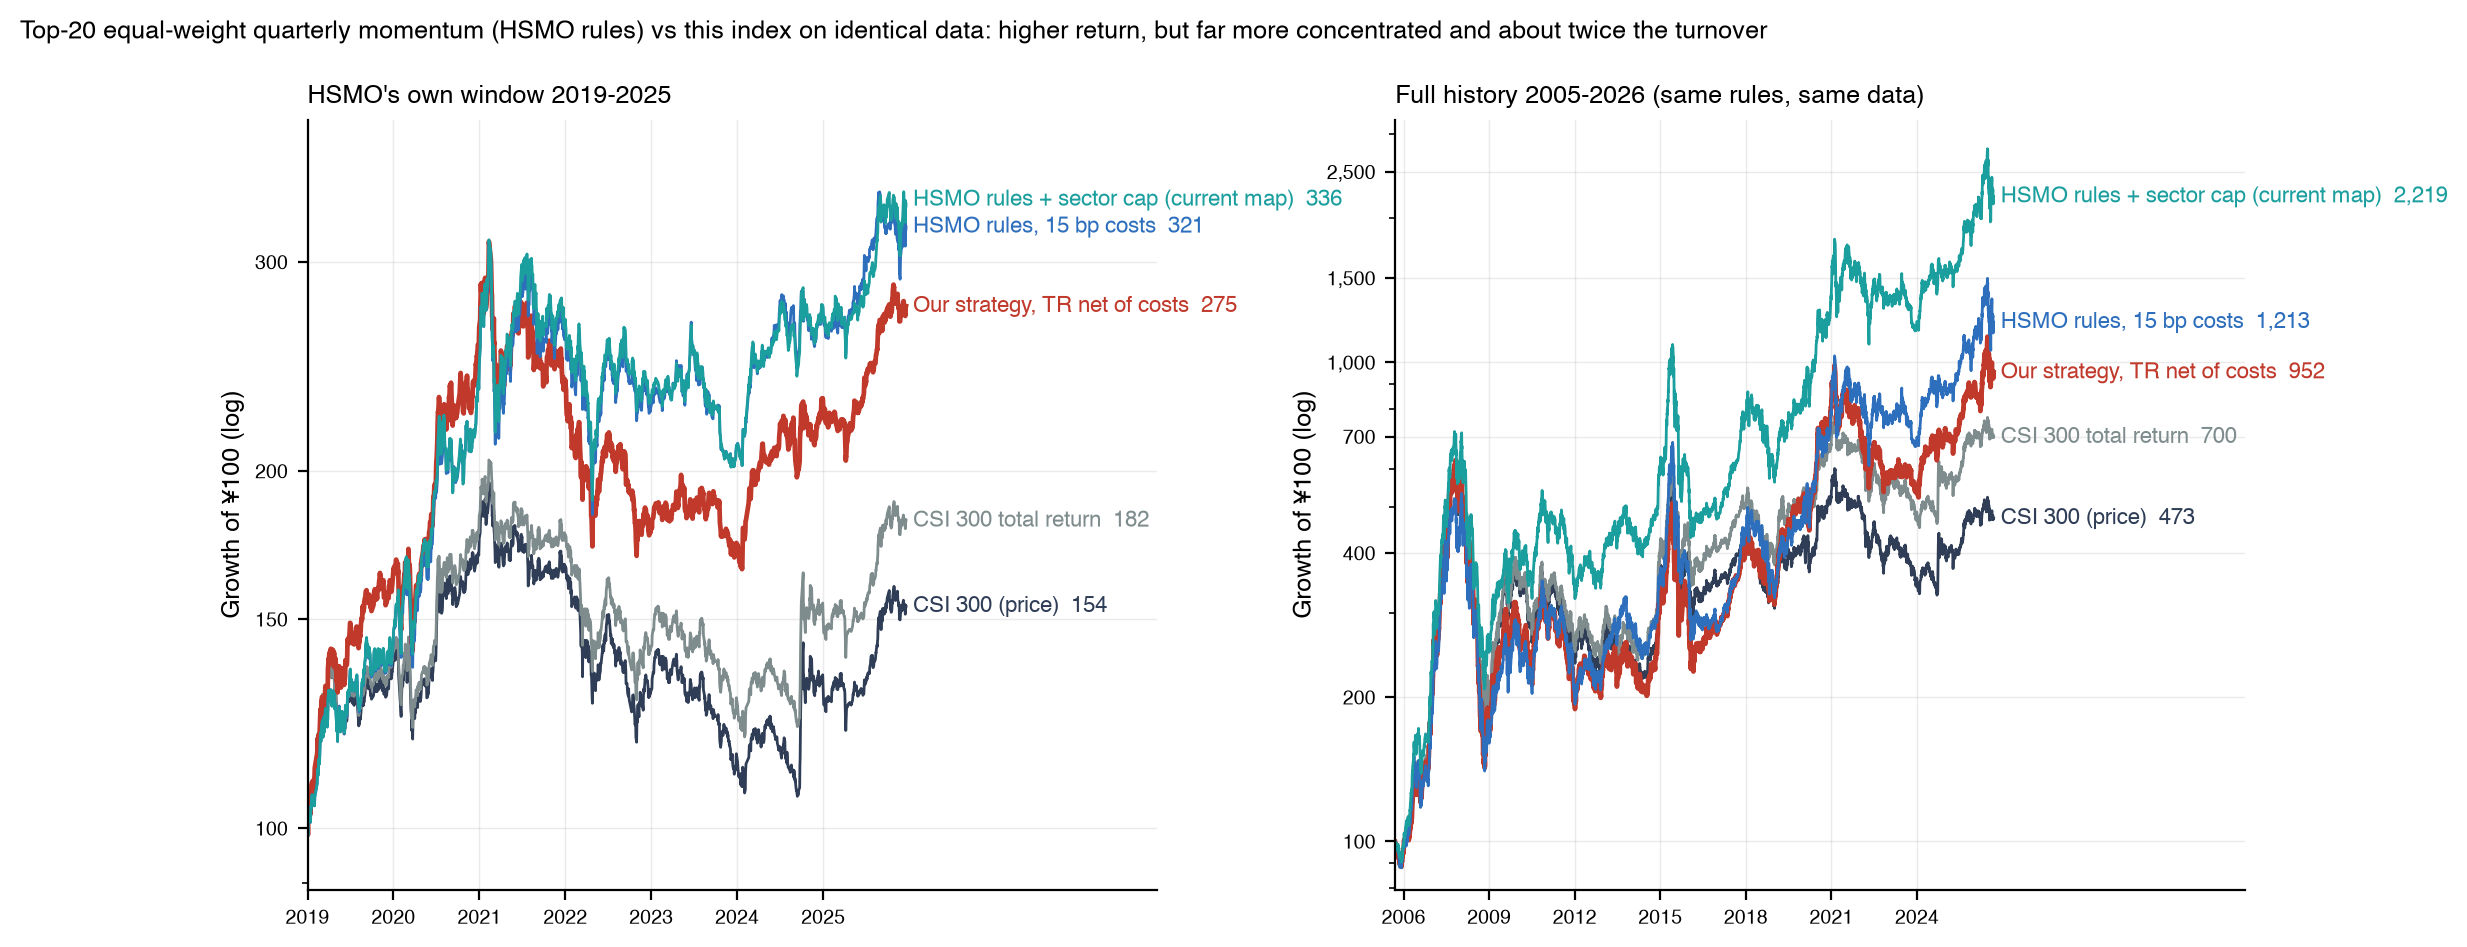
\includegraphics[width=\textwidth]{../charts/research/rr_hsmo_comparison.png}
\caption{HSMO 规则（在本文数据上复现）与本指数：其 2019--2025 年窗口（左）与 2005--2026 年全样本（右），\textyen 100，对数坐标}\label{fig:hsmo}
\end{figure}

\begin{figure}[!htbp]
\centering
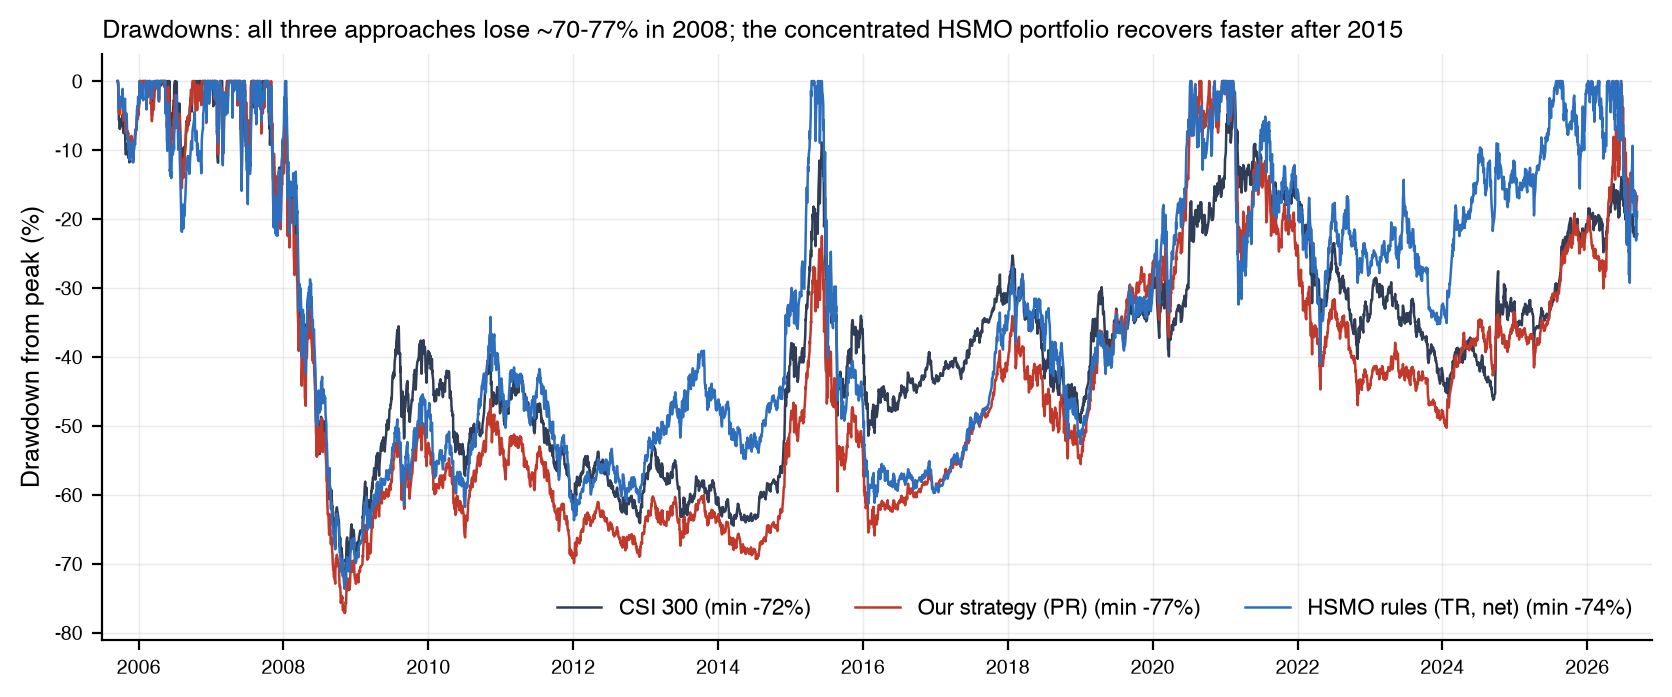
\includegraphics[width=\textwidth]{../charts/research/rr_drawdown_comparison.png}
\caption{回撤比较：沪深300、本指数（价格）、HSMO 规则（全收益、费后）}\label{fig:dd3}
\end{figure}

\FloatBarrier
\subsection{评述}
两种设计代表了动量因子的两种用法。HSI300-Momentum-Strategy 是\textbf{高活跃度的因子组合}：更集中、更快的调仓让它在趋势切换后能更早转向，历史收益更高，但波动、换手、成本和单一行业与个股风险也更高，且其点位数据（月末快照、当前行业分类）与成本假设（15\,bp）在 2005--2008 年的制度环境下偏乐观。本文是\textbf{可指数化的规则}：更宽的成分、市值倾斜的权重、缓冲和上限带来更低的换手和更接近母指数的风险特征（$\beta\approx 1$、跟踪误差约 10\%），代价是对趋势反转反应更慢（2021 年、2024 年 9 月）。两者在同一数据上都长期战胜沪深300，也都在 2008、2011、2015--2016 年经历长时间跑输——\textbf{动量在 A 股大盘股中的有效性是周期性的}，任何以 2019 年以后样本为依据的收益预期都需要打折。
\section{结论}\label{sec:conclusion}
把 S\&P 500 Momentum 的规则平移到沪深300并叠加 Financial Viability 盈利资格，在 2005--2026 年得到一条\textbf{长期期望为正、但需要忍受多年跑输}的规则：年化收益由 7.68\% 提高到 9.83\%（费后 9.33\%），Sharpe 由 0.43 升至 0.49，但波动与最大回撤更大，超额收益集中在 2017--2020 年，月度超额在统计上不显著。超额几乎全部来自选股而非 SPMO 式加权；本文的自由流通代理对国有大盘股的高配使报告的业绩偏保守。相同数据上，更集中、更高频的 Top-20 等权季度动量收益更高，但换手约两倍、集中度更高，其行业中性规则依赖当前分类而在历史上不可靠。研究任务书要求回答的 17 个问题逐条如下。
\begin{enumerate}[leftmargin=2em,itemsep=2pt]
\item \textbf{回测起止日期}\quad 2005-09-16 至 2026-09-09（首个参考日 2005-08-31，首次实施 2005-09-16；22 个日历年，含首尾不完整年份）。
\item \textbf{\textyen 100 投资沪深300}\quad \textyen472.6（价格指数）；含股息 \textyen700.1。
\item \textbf{\textyen 100 投资策略}\quad \textyen715.6（费前）/ \textyen649.8（费后）；全收益费前 \textyen1,051.8。
\item \textbf{两者 CAGR}\quad 沪深300 7.68\%，策略 9.83\%（全收益口径 9.72\% 对 11.87\%）。
\item \textbf{策略年化超额收益}\quad 2.15\%（费后 1.65\%）；Jensen $\alpha$ 2.62\%，$\beta$ 0.99。
\item \textbf{两者最大回撤}\quad 沪深300 $-$72.30\%（2007-10-16 $\rightarrow$ 2008-11-04）；策略 $-$77.16\%（2007-10-31 $\rightarrow$ 2008-11-04）。
\item \textbf{两者 Sharpe}\quad 沪深300 0.43，策略 0.49（费后 0.47）。
\item \textbf{两者年化波动率}\quad 沪深300 24.69\%，策略 26.71\%。
\item \textbf{策略平均换手率}\quad 单边每次调仓 55.1\%，每年 107.7\%（最高单次 82.8\%）。
\item \textbf{扣除交易成本后的策略 CAGR}\quad 9.33\%（成本拖累 0.50\%/年）。
\item \textbf{策略最强的年份}\quad 2007 年（+168.5\%）、2006 年（+113.0\%）、2009 年（+75.5\%）；超额最大：2020 年（+33.0\%）、2019 年（+23.4\%）、2017 年（+22.7\%）。
\item \textbf{策略最差的年份}\quad 2008 年（$-$69.0\%）、2011 年（$-$34.2\%）、2022 年（$-$27.0\%）；超额最差：2009 年（$-$21.2\%）、2014 年（$-$14.4\%）、2015 年（$-$13.1\%）。
\item \textbf{最大 Momentum Crash}\quad 2024-08-27 至 2024-12-03，策略 $-$3.1\% 对沪深300 +19.6\%（相对 $-$22.7\%）。
\item \textbf{是否长期稳定跑赢沪深300}\quad 长期跑赢但不稳定：22 年中 12 年跑赢，2005--2016 年累计跑输且相对强度回撤 $-$33.2\%、历时 3130 天，超额几乎全部来自 2017 年以后；月度超额的 $t$ 统计量 0.97，统计上不显著。
\item \textbf{3 年和 5 年滚动超额收益胜率}\quad 3 年 60.4\%，5 年 61.4\%（1 年 56.4\%）。
\item \textbf{相对强度长期趋势}\quad 由 1.00 升至 1.51（年化 +2.00\%），但先经历 2007--2016 年的长期下行（$-$33.2\%），2017 年后转为上行并于 2019 年收复。
\item \textbf{Financial Viability + SPMO 是否显著改善沪深300的长期复利与风险调整收益}\quad 长期复利有实质改善（年化 7.68\% $\rightarrow$ 9.83\%，费后 9.33\%；21 年终值高 51\%），风险调整收益温和改善（Sharpe 0.43 $\rightarrow$ 0.49，Sortino 0.59 $\rightarrow$ 0.68，信息比率 0.20），但波动和最大回撤更大、超额收益集中在少数年份且统计上不显著。结论：\textbf{有改善，但不能称为“显著”}。
\end{enumerate}
\begin{thebibliography}{99}\footnotesize
\bibitem[Jegadeesh and Titman(1993)]{jegadeesh1993} Jegadeesh, N., and S. Titman. 1993. Returns to Buying Winners and Selling Losers: Implications for Stock Market Efficiency. \emph{Journal of Finance} 48(1): 65--91.
\bibitem[Carhart(1997)]{carhart1997} Carhart, M. M. 1997. On Persistence in Mutual Fund Performance. \emph{Journal of Finance} 52(1): 57--82.
\bibitem[Asness et al.(2013)]{asness2013} Asness, C. S., T. J. Moskowitz, and L. H. Pedersen. 2013. Value and Momentum Everywhere. \emph{Journal of Finance} 68(3): 929--985.
\bibitem[Daniel and Moskowitz(2016)]{daniel2016} Daniel, K., and T. J. Moskowitz. 2016. Momentum Crashes. \emph{Journal of Financial Economics} 122(2): 221--247.
\bibitem[Barroso and Santa-Clara(2015)]{barroso2015} Barroso, P., and P. Santa-Clara. 2015. Momentum Has Its Moments. \emph{Journal of Financial Economics} 116(1): 111--120.
\bibitem[S\&P Dow Jones Indices(2026a)]{spdji_momentum} S\&P Dow Jones Indices. 2026. \emph{S\&P Momentum Indices Methodology}. New York: S\&P Global.
\bibitem[S\&P Dow Jones Indices(2026b)]{spdji_us} S\&P Dow Jones Indices. 2026. \emph{S\&P U.S. Indices Methodology}. New York: S\&P Global.
\bibitem[S\&P Dow Jones Indices(2015)]{spdji_bovespa} S\&P Dow Jones Indices. 2015. \emph{S\&P/BOVESPA Momentum Index Methodology}. New York: S\&P Global.
\bibitem[中证指数有限公司(2026)]{csindex} 中证指数有限公司. 2026. 《沪深300指数编制方案》及历次样本调整公告. \url{https://www.csindex.com.cn}.
\bibitem[HSI300-Momentum-Strategy(2025)]{hsmo} dongzhaohe321418-lab. 2025. \emph{HSI300-Momentum-Strategy}: 沪深300 Top-20 等权季度动量策略. GitHub. \url{https://github.com/dongzhaohe321418-lab/HSI300-Momentum-Strategy}.
\end{thebibliography}
\appendix
\section{最新持仓与待实施名单}\label{app:holdings}
{\scriptsize
\begin{longtable}{@{}llrrrrl@{}}
\caption{2026-03-20 实施（参考日 2026-02-27）的全部 55 只成分股}\label{tab:holdings}\\
\toprule
代码 & 名称 & Score & 排名 & 沪深300权重（代理） & 最终权重 & 触及上限 \\
\midrule
\endfirsthead
\toprule
代码 & 名称 & Score & 排名 & 沪深300权重（代理） & 最终权重 & 触及上限 \\
\midrule
\endhead
\bottomrule
\endfoot
\endlastfoot
601138 & 工业富联 & 3.03 & 13 & 2.12\% & 9.00\% & 是 \\
601288 & 农业银行 & 1.79 & 48 & 3.92\% & 9.00\% & 是 \\
601899 & 紫金矿业 & 3.73 & 7 & 1.56\% & 8.71\% &  \\
300308 & 中际旭创 & 4.00 & 1 & 1.13\% & 6.76\% &  \\
603993 & 洛阳钼业 & 4.00 & 3 & 0.80\% & 4.80\% &  \\
300502 & 新易盛 & 4.00 & 5 & 0.61\% & 3.65\% &  \\
688041 & 海光信息 & 1.99 & 42 & 1.16\% & 3.46\% &  \\
300476 & 胜宏科技 & 4.00 & 4 & 0.50\% & 2.98\% &  \\
601318 & 中国平安 & 1.52 & 61 & 1.29\% & 2.92\% &  \\
688256 & 寒武纪 & 2.01 & 41 & 0.95\% & 2.84\% &  \\
002371 & 北方华创 & 2.21 & 32 & 0.66\% & 2.16\% &  \\
300394 & 天孚通信 & 2.42 & 26 & 0.55\% & 1.98\% &  \\
600111 & 北方稀土 & 2.93 & 16 & 0.43\% & 1.89\% &  \\
000792 & 盐湖股份 & 3.11 & 10 & 0.39\% & 1.80\% &  \\
688008 & 澜起科技 & 3.01 & 14 & 0.36\% & 1.61\% &  \\
000408 & 藏格矿业 & 4.00 & 2 & 0.26\% & 1.55\% &  \\
600489 & 中金黄金 & 3.50 & 8 & 0.30\% & 1.55\% &  \\
603986 & 兆易创新 & 2.59 & 19 & 0.38\% & 1.49\% &  \\
603799 & 华友钴业 & 3.44 & 9 & 0.28\% & 1.46\% &  \\
300274 & 阳光电源 & 2.17 & 34 & 0.44\% & 1.43\% &  \\
600547 & 山东黄金 & 2.89 & 17 & 0.33\% & 1.42\% &  \\
688012 & 中微公司 & 2.17 & 33 & 0.42\% & 1.37\% &  \\
002916 & 深南电路 & 2.50 & 22 & 0.36\% & 1.36\% &  \\
600089 & 特变电工 & 3.08 & 11 & 0.29\% & 1.35\% &  \\
600362 & 江西铜业 & 3.87 & 6 & 0.23\% & 1.33\% &  \\
603259 & 药明康德 & 1.84 & 45 & 0.47\% & 1.28\% &  \\
600346 & 恒力石化 & 2.33 & 27 & 0.35\% & 1.21\% &  \\
600183 & 生益科技 & 2.44 & 23 & 0.32\% & 1.16\% &  \\
002028 & 思源电气 & 3.03 & 12 & 0.25\% & 1.14\% &  \\
601600 & 中国铝业 & 2.02 & 40 & 0.35\% & 1.04\% &  \\
601336 & 新华保险 & 2.23 & 30 & 0.30\% & 1.00\% &  \\
600031 & 三一重工 & 1.74 & 50 & 0.38\% & 0.97\% &  \\
601698 & 中国卫通 & 2.09 & 37 & 0.30\% & 0.94\% &  \\
000338 & 潍柴动力 & 2.33 & 28 & 0.27\% & 0.93\% &  \\
002493 & 荣盛石化 & 1.96 & 43 & 0.28\% & 0.82\% &  \\
601100 & 恒立液压 & 1.88 & 44 & 0.29\% & 0.81\% &  \\
000807 & 云铝股份 & 2.54 & 21 & 0.21\% & 0.79\% &  \\
000630 & 铜陵有色 & 3.00 & 15 & 0.17\% & 0.76\% &  \\
600176 & 中国巨石 & 2.44 & 24 & 0.21\% & 0.76\% &  \\
002384 & 东山精密 & 2.07 & 39 & 0.23\% & 0.70\% &  \\
002463 & 沪电股份 & 1.48 & 64 & 0.31\% & 0.68\% &  \\
000975 & 山金国际 & 2.75 & 18 & 0.15\% & 0.62\% &  \\
000776 & 广发证券 & 1.66 & 55 & 0.24\% & 0.58\% &  \\
600160 & 巨化股份 & 1.80 & 47 & 0.22\% & 0.58\% &  \\
600426 & 华鲁恒升 & 2.42 & 25 & 0.16\% & 0.57\% &  \\
002600 & 领益智造 & 1.72 & 51 & 0.21\% & 0.55\% &  \\
600219 & 南山铝业 & 2.29 & 29 & 0.16\% & 0.53\% &  \\
002466 & 天齐锂业 & 2.22 & 31 & 0.16\% & 0.53\% &  \\
600522 & 中天科技 & 1.76 & 49 & 0.19\% & 0.50\% &  \\
600875 & 东方电气 & 2.08 & 38 & 0.16\% & 0.50\% &  \\
000425 & 徐工机械 & 1.57 & 60 & 0.21\% & 0.50\% &  \\
002709 & 天赐材料 & 2.56 & 20 & 0.12\% & 0.47\% &  \\
688082 & 盛美上海 & 2.13 & 36 & 0.14\% & 0.46\% &  \\
002074 & 国轩高科 & 2.16 & 35 & 0.13\% & 0.41\% &  \\
300803 & 指南针 & 1.84 & 46 & 0.13\% & 0.37\% &  \\
\bottomrule
\end{longtable}
}

{\scriptsize
\begin{longtable}{@{}llrrr@{}}
\caption{参考日 2026-08-31 已计算、将于 2026-09-18 收盘后实施的 54 只（未进入回测）}\label{tab:pending}\\
\toprule
代码 & 名称 & Score & 排名 & 目标权重 \\
\midrule
\endfirsthead
\toprule
代码 & 名称 & Score & 排名 & 目标权重 \\
\midrule
\endhead
\bottomrule
\endfoot
\endlastfoot
300308 & 中际旭创 & 4.00 & 2 & 9.00\% \\
300750 & 宁德时代 & 2.03 & 40 & 8.49\% \\
601138 & 工业富联 & 1.78 & 50 & 6.20\% \\
688256 & 寒武纪 & 2.49 & 20 & 4.72\% \\
601899 & 紫金矿业 & 2.29 & 28 & 4.29\% \\
300502 & 新易盛 & 3.08 & 12 & 4.20\% \\
002371 & 北方华创 & 2.84 & 14 & 3.90\% \\
688041 & 海光信息 & 2.20 & 30 & 3.52\% \\
000333 & 美的集团 & 2.08 & 37 & 3.40\% \\
688012 & 中微公司 & 3.19 & 11 & 2.95\% \\
600183 & 生益科技 & 2.82 & 15 & 2.83\% \\
603986 & 兆易创新 & 3.53 & 8 & 2.60\% \\
603993 & 洛阳钼业 & 2.74 & 17 & 2.47\% \\
002384 & 东山精密 & 3.22 & 10 & 2.40\% \\
300408 & 三环集团 & 3.96 & 4 & 2.30\% \\
688072 & 拓荆科技 & 4.00 & 1 & 2.08\% \\
002475 & 立讯精密 & 1.81 & 48 & 2.07\% \\
600176 & 中国巨石 & 3.82 & 6 & 1.81\% \\
002415 & 海康威视 & 1.96 & 42 & 1.72\% \\
688008 & 澜起科技 & 2.63 & 18 & 1.67\% \\
300394 & 天孚通信 & 2.14 & 35 & 1.66\% \\
603259 & 药明康德 & 1.55 & 62 & 1.61\% \\
002916 & 深南电路 & 2.41 & 24 & 1.60\% \\
601872 & 招商轮船 & 3.47 & 9 & 1.42\% \\
002463 & 沪电股份 & 2.00 & 41 & 1.30\% \\
301308 & 江波龙 & 3.95 & 5 & 1.15\% \\
301165 & 锐捷网络 & 2.76 & 16 & 1.06\% \\
002353 & 杰瑞股份 & 4.00 & 3 & 0.98\% \\
600989 & 宝丰能源 & 1.93 & 43 & 0.95\% \\
688082 & 盛美上海 & 2.38 & 25 & 0.93\% \\
605117 & 德业股份 & 3.01 & 13 & 0.91\% \\
000657 & 中钨高新 & 3.53 & 7 & 0.91\% \\
000338 & 潍柴动力 & 2.42 & 22 & 0.88\% \\
000408 & 藏格矿业 & 2.44 & 21 & 0.81\% \\
600584 & 长电科技 & 2.15 & 34 & 0.79\% \\
600522 & 中天科技 & 2.42 & 23 & 0.79\% \\
600188 & 兖矿能源 & 2.04 & 39 & 0.78\% \\
000792 & 盐湖股份 & 1.89 & 45 & 0.76\% \\
601100 & 恒立液压 & 1.76 & 51 & 0.66\% \\
600489 & 中金黄金 & 1.87 & 47 & 0.63\% \\
600362 & 江西铜业 & 2.29 & 27 & 0.62\% \\
002028 & 思源电气 & 2.61 & 19 & 0.60\% \\
002493 & 荣盛石化 & 1.58 & 56 & 0.60\% \\
000988 & 华工科技 & 2.06 & 38 & 0.59\% \\
000807 & 云铝股份 & 2.15 & 33 & 0.55\% \\
600549 & 厦门钨业 & 2.34 & 26 & 0.53\% \\
600160 & 巨化股份 & 1.78 & 49 & 0.53\% \\
600089 & 特变电工 & 1.89 & 46 & 0.49\% \\
600118 & 中国卫星 & 2.19 & 31 & 0.42\% \\
000630 & 铜陵有色 & 2.09 & 36 & 0.42\% \\
600026 & 中远海能 & 1.93 & 44 & 0.38\% \\
002001 & 新和成 & 1.71 & 52 & 0.38\% \\
002202 & 金风科技 & 2.16 & 32 & 0.36\% \\
002709 & 天赐材料 & 2.20 & 29 & 0.33\% \\
\bottomrule
\end{longtable}
}

\section{参数与输出文件}
\begin{table}[!htbp]
\centering
\small
\caption{策略参数（\texttt{config.yaml}，未做任何收益导向调整）}\label{tab:params}
\begin{tabular}{@{}p{3.2cm}p{11.8cm}@{}}
\toprule
参数 & 取值 \\
\midrule
Financial Viability & 最近一季 $>0$ 且最近四季合计 $>0$；字段 \texttt{CONTINUED\_NETPROFIT} → \texttt{NETPROFIT}；公告日 $\leq$ 参考日；不合理公告日 → 法定截止日 \\
动量窗口 & 参考日前 13 个月 → 前 1 个月；最少 150 个交易日 \\
$Z$ 分数截断 & $\pm 3$ \\
选样比例 & 合格股票的 20\%（四舍五入） \\
缓冲 & 前 80\% 自动入选；现成分股 120\% 以内保留 \\
权重上限 & $\min(9\%,\,20\,w^P)$；无可行解时倍数逐步加 1（本次运行未触发） \\
调仓 & 2 / 8 月最后一个交易日参考；3 / 9 月第三个星期五收盘后实施 \\
成本 & 佣金、印花税、过户费按历史制度；冲击成本固定 0.10\% 每边 \\
指数基点 & 1000（绩效比较按 \textyen 100 重设） \\
\bottomrule
\end{tabular}
\end{table}

\begin{table}[!htbp]
\centering
\footnotesize
\caption{主要输出文件}\label{tab:files}
\begin{tabular}{@{}p{7.4cm}p{7.6cm}@{}}
\toprule
文件 & 内容 \\
\midrule
output/scores/YYYY-MM-DD.csv & 每个参考日全部沪深300成分股的资格、动量、$Z$ 分数、Momentum Score、排名、权重 \\
output/holdings/YYYY-MM-DD.csv & 每次实施的成分股与权重（\texttt{\_pending} 为尚未实施） \\
output/performance/index\_levels.csv & 日频指数点位：沪深300、策略（费前 / 费后）、全收益版本 \\
output/performance/strategy\_ohlc.csv, csi300\_ohlc.csv & 日 OHLC（策略成交量留空） \\
output/performance/*.csv & 统计、周期、崩塌、调仓摘要与资格审计 \\
output/research/*.csv & 本文的归因、HSMO 复现、集中度、漏斗、持续性、行业暴露分析表 \\
data/processed/csi300\_membership\_intervals.csv & 点位成分股区间表（949 只证券） \\
\bottomrule
\end{tabular}
\end{table}

\end{document}